%!TEX root = ../thesis.tex
%*******************************************************************************
%****************************** Third Chapter **********************************
%*******************************************************************************
\chapter{Latent Space Learning Theory}\label{chapter:latent-space-learning-theory}

% **************************** Define Graphics Path **************************
\ifpdf
    \graphicspath{{Chapter5/Figs/Raster/}{Chapter5/Figs/PDF/}{Chapter5/Figs/}}
\else
    \graphicspath{{Chapter5/Figs/Vector/}{Chapter5/Figs/}}
\fi

\emph{This chapter presents and analyses RAM-MC, an f-divergence estimator that is applicable to estimating divergences between particular distributions in the latent spaces of autoencoder models such as Variational Autoencoders and Wasserstein Autoencoders. 
Learning theoretic analyses of sampled-based $f$-divergence estimators usually yield poor rates of convergence unless strong assumptions are made.
By exploiting the natural structure present in the autoencoder setting, RAM-MC exhibits fast rates under mild assumptions.}

\emph{This work is an important contribution to the literature for two main reasons. 
First, it demonstrates that the $f$-divergences considered can be estimated with a practical number of samples.
Second, it provides a rigorous foundation to heuristically proposed methods for estimating and minimising Total Correlation and Mutual Information in the context of Variational Autoencoders.}

\emph{The main technical content of this chapter has been published in the paper:}

\begin{quote}
\fullcite{rubenstein2019practical}
\end{quote}

%\emph{Additionally, the following related workshop papers were published during my PhD but are not included in this thesis:}
%
%\begin{quote}
%\fullcite{rubenstein2018wasserstein}
%\end{quote}
%
%\begin{quote}
%\fullcite{rubenstein2018learning}
%\end{quote}
%
%\emph{The main contribution of this chapter is a learning theoretic analysis of estimating divergences between distributions. 
%The setting considered by this work occurs naturally in and has application to the latent variable models used in the generative modelling community, in particular Wasserstein Autoencoders.
%Sections ?? - ?? are a review of generative modelling, setting the stage for Sections ?? - ?? which is based on} \cite{rubenstein2019practical}.
%
%\todo{replace $D(.\|.)$ with $D(.,.)$}

%\todo{Consistent use of -divergence and whether $H^2$ is italicised or not}

\section{Introduction}

The estimation and minimisation of divergences between probability distributions based on samples are fundamental problems of machine learning.
The previous chapter discussed generative modelling, but there are numerous other applications across the literature.
For example, 
%maximum likelihood learning can be viewed as minimizing the Kullback-Leibler divergence $D_{\text{KL}}(P_{\text{data}}, P_{\text{model}})$ with respect to the model parameters.
%More generally, generative modelling
%%---most famously Variational Autoencoders and Generative Adversarial Networks \cite{kingma2013auto, goodfellow2014generative} discussed in the next section---
%can be viewed as minimizing a divergence $\smash{D(P_{\text{data}}, P_{\text{model}})}$ where $\smash{P_{\text{model}}}$ may be intractable.
in variational inference, an intractable posterior $p(z|x)$ is approximated with a tractable distribution $q(z)$ chosen to minimise the Kullback-Leibler ($\KL$) divergence $\smash{D_{\text{KL}}\bigl(q(z) , p(z|x)\bigr)}$.
The mutual information between two variables $\smash{I(X,Y)}$, core to information theory and Bayesian machine learning, is equivalent to $\smash{D_{\text{KL}}(P_{X,Y} , P_X P_Y)}$. 
Independence testing often involves estimating a divergence $\smash{D(P_{X,Y} , P_X P_Y)}$, while two-sample testing (does $P=Q$?) involves estimating a divergence $D(P,Q)$.
Additionally, one approach to domain adaptation, in which a classifier is learned on a distribution $P$ but tested on a distinct distribution $Q$, involves learning a feature map $\phi$ such that a divergence $\smash{D\left( \phi_\# P , \phi_\# Q \right)}$ is minimised, where $\smash{\phi_\#}$ represents the push-forward operation \citep{ben2007analysis,ganin2016domain}.

This chapter concerns the estimation of $f$-divergences, introduced in Section \ref{subsec:f-divergences-intro}.
%This chapter considers the well-known family of $f$-divergences \cite{csiszar2004information, liese2006divergences} that includes amongst others the $\KL$, Jensen-Shannon ($\JS$), $\chi^2$, and $\alpha$-divergences as well as the Total Variation ($\TV$) and squared Hellinger ($\Hsq$) distances, the latter two of which play an important role in the statistics literature \cite{tsybakov2009}.
A significant body of work exists studying estimation of $D_f(P , Q)$ for general probability distributions $P$ and $Q$.
While the majority of this focuses on $\alpha$-divergences and closely related R\'enyi-$\alpha$ divergences \citep{poczos11alpha, singh14alpha, krishnamurthy14icml},
many works address specifically the KL-divergence \citep{perez08kl, wang09kl}
with fewer considering $f$-divergences in full generality \citep{nguyen10ratio, kanamori12ratio, moon14ensemble, moon14followup}.
Although the $\KL$-divergence is the most frequently encountered $f$-divergence in the machine learning literature, in recent years there has been growing interest in other $f$-divergences \citep{nowozin2016f,zhang2019variational}, 
in particular in the variational inference community where they have been employed to derive alternative evidence lower bounds \citep{li2016renyi, dieng2017variational, pmlr-v80-chen18k}.


The main challenge in computing $D_f(P , Q)$ is that it requires knowledge of either both densities $p(x)$ and $q(x)$, or the density ratio $p(x)/q(x)$.
In studying this problem, assumptions of differing strength can be made about $P$ and $Q$. 
In the weakest \emph{agnostic} setting, one may be given only a finite number of \iid~samples from the distributions without any further knowledge of their densities.
As an example of stronger assumptions,
both distributions may be mixtures of Gaussians \citep{hershey2007approximating, durrieu2012lower}, 
or one may have access to samples from $Q$ and have full knowledge of $P$ as in e.g.~model fitting \citep{heroma2001techrep, heroma2002ieee}.

Most of the literature on $f$-divergence estimation considers the weaker agnostic setting.
The lack of assumptions makes such work widely applicable, but comes at the cost of needing to work around estimation of either the densities $p(x)$ and $q(x)$ \citep{singh14alpha, krishnamurthy14icml} or the density ratio $p(x)/q(x)$ \citep{nguyen10ratio, kanamori12ratio} from samples.
Both of these estimation problems are provably hard \citep{tsybakov2009, nguyen10ratio} and suffer rates---the speed at which the error of an estimator decays as a function of the number of samples $N$---of order $\smash{N^{-1/d}}$ when $P$ and $Q$ are defined over $\R^d$ unless their densities are sufficiently smooth.
This is a manifestation of the \emph{curse of dimensionality} and rates of this type are often called \emph{nonparametric}.
One could hope to estimate $D_f(P,Q)$ without explicitly estimating the densities or their ratio and thus avoid suffering nonparametric rates, however a lower bound of the same order $\smash{N^{-1/d}}$ is known for $\alpha$-divergences \citep{krishnamurthy14icml}, a sub-family of $f$-divergences.
While some works considering the agnostic setting provide rates for the bias and variance of the proposed estimator \citep{nguyen10ratio, krishnamurthy14icml} or even exponential tail bounds \citep{singh14alpha},
it is more common to only show that the estimators are asymptotically unbiased or consistent without proving specific rates of convergence \citep{wang09kl, poczos11alpha, kanamori12ratio}.


Motivated by recent advances in machine learning, this chapter considers a setting in which structural assumptions are made about the distributions.
Although the assumptions are strong, they are naturally satisfied in the setting of autoencoders with probabilistic encoders, including Wasserstein Autoencoders and variants of Variational Autoencoders.

\subsection{Summary of setting and results}

Let $\X$ and $\Z$ be two finite dimensional Euclidean spaces.
This chapter studies estimation of the divergence $D_f(Q_Z, P_Z)$ between two probability distributions $P_Z$ and $Q_Z$, both defined over $\Z$.
It is assumed that $P_Z$ has known density $p(z)$, while $Q_Z$ with density  $q(z)$ admits the factorization $\smash{q(z) = \int q(z|x)q(x) dx}$.
Access to independent samples from the distribution $Q_X$ with unknown density $q(x)$ and full knowledge of the conditional distribution $\smash{Q_{Z|X}}$ with density $q(z|x)$ are assumed.
%The true density $q(z)$ is unknown due to the integral over the unknown $q(x)$ and so is $D_f(Q_Z , P_Z)$.
In the language of autoencoders,
%As a concrete example, these assumptions are often satisfied in applications of modern unsupervised generative modeling with deep autoencoder architectures,
%where 
$\X$ and $\Z$ would be \emph{data} and \emph{latent} spaces, $\smash{P_Z}$ the \emph{prior}, $\smash{Q_X}$ the \emph{data distribution}, $\smash{Q_{Z|X}}$ the \emph{encoder}, and $\smash{Q_Z}$ the \emph{aggregate posterior}, though the theory presented in this work does not apply exclusively to this setting.

Given independent observations $\smash{X_1, \ldots, X_N}$ from $\smash{Q_X}$, the goal is to estimate $\smash{D_f(Q_Z , P_Z)}$.
The main contribution of this chapter is to use the finite mixture $\smash{\hat{Q}_Z^N := \frac{1}{N} \sum_{i=1}^N Q_{Z|X_i}}$ as a surrogate for the continuous mixture $\smash{Q_Z}$, 
to use this to approximate $\smash{D_f(Q_Z , P_Z)}$ with $\smash{D_f(\hat{Q}_Z^N , P_Z)}$,
%a quantity that can be estimated to arbitrary precision using Monte-Carlo sampling since both distributions have known densities, 
and to theoretically study conditions under which this approximation is reasonable.


$\smash{D_f(\hat{Q}_Z^N , P_Z)}$ is denoted the \emph{Random Mixture (RAM)} estimator and rates at which it converges to $\smash{D_f(Q_Z , P_Z)}$ as $N$ grows are derived.
Similar guarantees are also provided for \emph{RAM-MC}, a practical Monte-Carlo based version of RAM.
By side-stepping the need to perform density estimation, one obtains \emph{parametric} rates of order $N^{-\gamma}$, where $\gamma$ is independent of the dimension (see Tables \ref{table:convergence} and \ref{table:concentration}), although the constants may still in general show exponential dependence on dimension.
This is in contrast to the agnostic setting where \emph{both} nonparametric rates and constants are exponential in dimension. 

These results have immediate implications to existing literature.
For the particular case of the $\KL$ divergence, a similar approach has been heuristically applied 
for estimation of mutual information \citep{poolevariational} and total correlation \citep{chen2018isolating} in the context of Variational Autoencoders.
Both works have application to representation learning, the latter in particular to disentangled representation learning. 
The results presented in this chapter thus provide strong theoretical grounding for these existing methods through rigorous analysis lacking in the original proposals.
In these works, the quantities being estimated and minimised are $D_{\KL}(Q_{Z,X}, Q_ZQ_X )$ and $D_{\KL}(Q_Z, \prod_{i} Q_{Z_i})$ respectively. 
Each of these quantities can be rewritten in terms of $\smash{D_{\KL}(Q_Z , P_Z)}$ and so RAM-MC can be used to estimate them.
In doing so, one recovers the estimators proposed by the authors, thus results concerning the convergence properties of RAM-MC transfer to results about their estimators.
See Section \ref{sec:applications} for details. 

Moreover, while this work considers estimation of $\smash{D_f(Q_Z , P_Z)}$, minimisation of this quantity is the key challenge in the training of Wasserstein Autoencoders (see Section \ref{subsec:chapter2-wae}). 
Preliminary experiments not included in this thesis did not find the proposed RAM-MC estimator to lead to improved training over existing methods, but future research could investigate this more thoroughly.

Section \ref{sec:f-div-background} presents known results from the literature on $f$-divergences and basic results in learning theory that are used in the proofs of novel results presented in this chapter.
%Since the setting we consider arises naturally in the study of autoencoder-based generative models, the following Section \ref{sec:generative-modelling-tour} provides an overview of the key concepts in the generative modelling literature in the context of this chapter.
Following this, Section \ref{sec:theory} introduces the RAM and RAM-MC estimators and presents the main theoretical results, including rates of convergence for the bias (Theorems~\ref{thm:fast-KL-rate} and \ref{thm:convergence-rate-general}) and tail bounds (Theorems \ref{thm:concentration} and \ref{thm:mc-variance}).
Section \ref{sec:experiments} validates the results in both synthetic and real-data experiments. 
Section \ref{sec:applications} discusses applications of these results to the literature, and 
Section \ref{sec:conclusion} concludes.
The results presented in Section \ref{sec:theory} have long proofs; short sketches are presented in the main text, while the full proofs can be found in Appendix \ref{chapter:appendix-latex-space-learning-theory}.


\section{Background results}\label{sec:f-div-background}

This section presents basic results from the literature that are used in the proofs of novel results in this chapter.
These include bounds relating different $f$-divergences, closed-form expressions for some $f$-divergences in the case of Gaussian probability distributions, and basic concentration inequalities. 
Proofs are omitted for referenced results.


\subsection{$f$-divergence bounds}

The results presented here are inequalities relating the values taken by $f$-divergences. 
These are mostly used in the proof of Theorem \ref{thm:fast-KL-rate}.
A comprehensive treatment of the relationships between different $f$-divergences can be found in \cite{tsybakov2009}, from which many of the results below are taken.

\medskip

\begin{lemma}[Lemma 2.4, \cite{tsybakov2009}]\label{lemma:f-div-hleqkl}
Let $A$ and $B$ be probability distributions. Then,
\begin{align*}
\Hsq(A, B) \leq \KL(A,B).
\end{align*}
\end{lemma}

\medskip

\begin{lemma}[Pinsker's inequality, Lemma 2.5, \cite{tsybakov2009}]\label{lemma:f-div-pinsker}
Let $A$ and $B$ be probability distributions. Then,
\begin{align*}
\TV(A,B)  \leq \sqrt{\frac{1}{2}\KL(A, B)}.
\end{align*}
\end{lemma}

\medskip

\begin{lemma}[Lemma 2.7, \cite{tsybakov2009}]\label{lemma:f-div-klleqchi}
Let $A$ and $B$ be probability distributions. Then,
\begin{align*}
\KL(A,B) \leq e^{\KL(A, B)} - 1 \leq \chi^2(A, B).
\end{align*}
\end{lemma}


\medskip

\begin{lemma}[Theorem 2, \cite{osterreicher2003new}]\label{lemma:f-div-betaleqtv}
Let $A$ and $B$ be probability distributions. For any value $\beta \geq 0$, there exists a scalar $\psi(\beta)$ such that
\begin{align*}
D_{f_\beta}(A,B) \leq \psi(\beta) \TV(A, B).
\end{align*}
\end{lemma}

\medskip


\begin{lemma}\label{lemma:hilbertian-triangle}
Suppose that $D_f^{\frac{1}{2}}$ satisfies the triangle inequality.
Let $A_N$ be a sequence of probability distributions, and let $B$ and $C$ be fixed probability distributions.
Then for any $\lambda>0$,
\begin{align*}
    D_f\left(A_N , C\right) - D_f\left(B , C\right) \leq (1+\lambda) D_f\left(A_N , B \right) +  \frac{1}{\lambda} D_f\left(B , C \right).
\end{align*}
If, furthermore, $D_f\left(A_N , B\right) = O\left( \frac{1}{N^k} \right)$ 
for some $k>0$, 
then
\begin{align*}
	D_f\left(A_N , C\right)  - D_f\left(B , C\right) = O\left( \frac{1}{N^{k/2}} \right).
\end{align*}
\end{lemma}
\begin{proof}
The first inequality follows from the triangle inequality applied to $D_f^{\frac{1}{2}}(A_N, C)$, and the fact that $2\sqrt{ab} \leq \lambda a + \frac{b}{\lambda}$ for ${a, b, \lambda>0}$.
The second inequality follows from the first by taking $\lambda = N^{-\frac{k}{2}}$.
\end{proof}


%\begin{align*}
%    D_f\left(\hat{Q}^N_Z , P_Z\right) - D_f\left(Q_{Z} , P_Z\right) \leq (1+\lambda) D_f\left(\hat{Q}^N_Z , Q_Z \right) +  \frac{1}{\lambda} D_f\left(Q_{Z} , P_Z \right)
%\end{align*}
%If, furthermore, $\E_{\XN}\left[ D_f\left(\hat{Q}^N_Z , Q_Z\right)\right] = O\left( \frac{1}{N^k} \right)$ 
%for some $k>0$, 
%then
%\begin{align*}
%    \E_{\XN}\left[ D_f\left(\hat{Q}^N_Z , P_Z\right) \right] - D_f\left(Q_{Z} , P_Z\right) = O\left( \frac{1}{N^{k/2}} \right)
%\end{align*}
%\end{lemma}
%\begin{proof}
%The first inequality follows from the triangle inequality for $D_f^{\frac{1}{2}}$ on $\hat{Q}^N_Z$ and $P_Z$, and the fact that $2\sqrt{ab} \leq \lambda a + \frac{b}{\lambda}$ for ${a, b, \lambda>0}$.
%The second inequality follows from the first by taking $\lambda = N^{-\frac{k}{2}}$.
%\end{proof}



\subsection{Closed-form expressions for $f$-divergences between Gaussians}\label{subsec:f-div-closed-form-gaussians}

The closed-form expressions for $f$-divergences presented here 
%This section presents closed-form expressions for $f$-divergences. 
are used for the experiments in Section \ref{sec:experiments}, as well as to understand cases in which the assumptions of all results hold in practical scenarios, discussed at the end of Section \ref{sec:theory}.



\medskip
 
\begin{lemma}[Exercise 1.6.11, \cite{pardo2005statistical}]
The KL-divergence between two $d$-variate Gaussians is
\begin{align*}
\KL\bigl( \mathcal{N}(\mu_1, \Sigma_1), 
\mathcal{N}(\mu_2, \Sigma_2)\bigr) = \frac{1}{2} \left( \text{tr}\left(\Sigma_2^{-1} \Sigma_1\right)
+ (\mu_2  - \mu_1)^\intercal \Sigma_2^{-1}(\mu_2 - \mu_1) - d + \log\frac{|\Sigma_2|}{|\Sigma_1|}
\right).
\end{align*}
\end{lemma}

\medskip

\begin{lemma}[Exercise 1.6.14, \cite{pardo2005statistical}]
The squared Hellinger ($H^2$) divergence between two multivariate Gaussians is
\begin{align*}
&\mathrm{H}^2\bigl( \mathcal{N}(\mu_1, \Sigma_1), 
\mathcal{N}(\mu_2, \Sigma_2)\bigr) \\
&\qquad = 1 - \frac{ \det (\Sigma_1)^{1/4} \det (\Sigma_2) ^{1/4}} { \det \left( \frac{\Sigma_1 + \Sigma_2}{2}\right)^{1/2} }
              \exp\left\{-\frac{1}{8}(\mu_1 - \mu_2)^T 
              \left(\frac{\Sigma_1 + \Sigma_2}{2}\right)^{-1}
              (\mu_1 - \mu_2)              
              \right\}.
\end{align*}
\end{lemma}


\medskip

%The closed form expression for the $\chi^2$-divergence between two $d$-variate normal distributions can be found in Lemma 1 of~\cite{NielsenN14}:
\begin{lemma}[Lemma 1, \cite{NielsenN14}]\label{lemma:chi-squared-closed-form}
Suppose that $P_1$ and $P_2$ are members of the same exponential family of distributions with log-partition function $F$ and natural parameters $\theta_1$ and $\theta_2$ respectively. Then
\begin{align*}
\chi^2(P_1, P_2) = e^{F(2\theta_2 - \theta_1) - \left(2F(\theta_2) - F(\theta_1) \right) } - 1,
\end{align*}
and is finite provided that $2\theta_2 - \theta_1$ belongs to the natural parameter space.
In the particular case of Gaussians,
\begin{align*}
\chi^2\bigl( \mathcal{N}(\mu_1, \Sigma_1), 
&\mathcal{N}(\mu_2, \Sigma_2)\bigr)
=
\frac{\mathrm{det}(\Sigma_2^{-1})}{\sqrt{\mathrm{det}(2\Sigma_2^{-1} - \Sigma_1^{-1})\mathrm{det}(\Sigma_1^{-1})}}
\exp\left(
\frac12\mu_2'\Sigma_1^{-1}\mu_2 
-\mu_1'\Sigma_2^{-1}\mu_1 
\right)\\
&\times\exp\left(
-\frac14(2\mu_1' \Sigma_2^{-1} - \mu_2' \Sigma_1^{-1})
\bigl(\frac12 \Sigma_1^{-1} - \Sigma_2^{-1}\bigr)^{-1}
(2\Sigma_2^{-1}\mu_1 - \Sigma_1^{-1}\mu_2)
\right) - 1.
\end{align*}
%\todo{in particular, this is finite when... ref assumptions section which uses this lemma.}
\end{lemma}
%As a corollary, the following also holds:
%\begin{corollary}
%Chi square divergence between two $d$-variate Gaussian distributions both having covariance matrices proportional to identity can be computed as:
%\[
%\chi^2\bigl( \mathcal{N}(\mu, \sigma^2 I_d), \mathcal{N}(0, \beta^2 I_d)\bigr)
%=
%\left(\frac{\beta^2}{\sigma^2\sqrt{2\beta^2/\sigma^2 - 1}}\right)^d
%e^{\frac{\|\mu\|^2}{2\beta^2 - \sigma^2}}
%- 1
%\]
%assuming $2\beta^{2} > \sigma^{2}$. 
%Otherwise the divergence is infinite.
%\end{corollary}


\subsection{Concentration inequalities}

Concentration inequalities provide bounds on the probability with which a random variable deviates from its expectation.
Here two such results are outlined; a comprehensive study can be found in \cite{boucheron2013concentration}. 
One basic result is \emph{Chebyshev's inequality}.

\medskip

\begin{lemma}[Chebyshev's inequality, Section 2.1, \cite{boucheron2013concentration}]\label{lemma:chebyshev}
Let $X$ be a random variable with finite expectation and variance. Then, for any $t>0$,
\begin{align*}
\mathbb{P}\left( |X - \mathbb{E}X | \geq t \right) \leq \frac{\mathrm{Var}(X)}{t}.
\end{align*}
\end{lemma}

A much stronger concentration result, \emph{McDiarmid's inequality} (sometimes called the \emph{bounded difference	inequality}), provides an exponential bound if the \emph{bounded difference property} is satisfied.
This result forms the basis of the proof of Theorem \ref{thm:concentration}.

\medskip

\begin{theorem}[McDiarmid's inequality, Theorem 6.2, \cite{boucheron2013concentration}]\label{thm:mcdiarmid}
Suppose that $X_1, \ldots, X_N \in \mathcal{X}$ are independent random variables and that $\phi : \mathcal{X}^N \to \R$ is a function. 
If it holds that for all $i\in\{1,\ldots,N\}$ and $x_1, \ldots, x_N, x_{i'}$, 
\begin{align*}
    \left| \phi(x_1, \ldots, x_{i-1}, x_i, x_{i+1}, \ldots, x_N) - \phi(x_1, \ldots, x_{i-1}, x_{i'}, x_{i+1}, \ldots, x_N)\right| \leq c_i,
\end{align*}
then
\begin{align*}
    \mathbb{P} \left(|\phi(X_1,\ldots, X_N) - \E\phi| \geq t \right) \leq 2\exp\left(\frac{-2t^2}{\sum_{i=1}^N c^2_i} \right).
\end{align*}
%\begin{align*}
%    \mathbb{P} \left(\phi(X_1,\ldots, X_N) - \E\phi \geq t \right) \leq \exp\left(\frac{-2t^2}{\sum_{i=1}^N c^2_i} \right)
%\end{align*}
%and
%\begin{align*}
%    \mathbb{P} \left(\phi(X_1,\ldots, X_N) - \E\phi \geq -t \right) \leq \exp\left(\frac{-2t^2}{\sum_{i=1}^N c^2_i} \right)
%\end{align*}
\end{theorem}




\section{Random mixture estimator and convergence results}\label{sec:theory}

This section introduces the proposed $f$-divergence estimator and presents theoretical guarantees for it.
The existence is assumed of probability distributions
${P_Z}$ and ${Q_Z}$ defined over $\Z$ with known density $p(z)$ and intractable density ${q(z) = \int q(z|x) q(x) dx}$ respectively,  where ${Q_{Z|X}}$ is known. 
$Q_X$ defined over $\X$ is unknown, but a set of i.i.d.\:samples ${\XN=\{X_1, \ldots, X_N\}}$ from $Q_X$ are given.
The ultimate goal is to estimate the $f$-divergence
%
\begin{align*}
    D_f(Q_Z , P_Z) = \int f \left( \frac{q(z)}{p(z)} \right) p(z) dz.
\end{align*}
%
This cannot be directly computed since $Q_Z$ is unknown. %intractable and so is ${D_f(Q_Z , P_Z)}$.
Substituting $Q_Z$ with a sample-based finite mixture ${\hat{Q}_Z^N := \frac{1}{N} \sum_{i=1}^N Q_{Z|X_i}}$ leads to the proposed 
\emph{Random Mixture estimator (RAM)}:
%
\begin{align}\textstyle
    D_f\bigl(\hat{Q}_Z^N , P_Z\bigr) := D_f\Big(\frac{1}{N} \sum_{i=1}^N Q_{Z|X_i} , P_Z\Big).
\end{align}
%
Although $\smash{\hat{Q}_Z^N} = \smash{\hat{Q}_Z^N}(\XN)$ is a function of the \iid~samples $\smash{\XN}$, this explicit dependence is omitted for notational brevity. 
The true $f$-divergence $D_f(Q_Z , P_Z)$ is a real-valued scalar, but $D_f\bigl(\hat{Q}_Z^N , P_Z\bigr)$ is a random variable whose randomness is inherited from the \iid~samples. 

The rest of this section is devoted to the exploration of conditions under which $\smash{D_f(\hat{Q}_Z^N , P_Z)}$ is a `good' estimator of $\smash{D_f(Q_{Z} , P_Z)}$.
More formally, conditions are established under which the estimator is asymptotically unbiased, concentrates to its expected value and can be practically estimated using Monte-Carlo sampling.

\subsection{Convergence rates for the bias of RAM}

The following proposition shows that $D_f(\hat{Q}_Z^N , P_Z)$ upper bounds $D_f(Q_{Z} , P_Z)$ in expectation for any finite $N$, and that the upper bound becomes tighter with increasing $N$. 
It follows that the \emph{bias} of RAM, the difference between its expectation and the true value of the quantity being estimated, is positive and decreasing in $N$.

\medskip

\begin{proposition}\label{prop:upper-bound}
Let $M \leq N$ be integers. Then
\begin{align}
\label{eq:our-estimate}
    D_f(Q_Z , P_Z) \ \leq 
    \mathbb{E}_{\mathbf{X}^N} \bigl[D_f(\hat{Q}_Z^N , P_Z)\bigr] \  \leq \ \mathbb{E}_{\mathbf{X}^M} \bigl[D_f(\hat{Q}_Z^M , P_Z)\bigr].
\end{align}
\end{proposition}
\begin{proof}[Proof sketch (full proof in Appendix \ref{proof:prop1})]
The first inequality follows from Jensen's inequality, using the facts that $f$ is convex and ${Q_Z = \E_{\XN} [\hat{Q}_Z^N}]$.
The second holds since a sample ${\XM}$ can be drawn by sub-sampling (without replacement) $M$ entries of ${\XN}$, and by applying Jensen's inequality again.
\end{proof}

As a function of $N$, the expectation of RAM is a decreasing sequence that is bounded below.
By the monotone convergence theorem, the sequence converges.
Theorems \ref{thm:fast-KL-rate} and \ref{thm:convergence-rate-general} below give sufficient conditions under which the expectation of RAM converges to $D_f(Q_{Z} , P_Z)$ as $N\to\infty$ for a variety of $f$s and provide rates at which this happens, summarised in Table \ref{table:convergence}.
The two theorems are proved using different techniques and assumptions. 
These assumptions, along with those of other methods (see Table~\ref{table:convergence-other}) are discussed in Section \ref{subsection:discussion-assumptions}.



\medskip


\begin{theorem}[Rates of the bias]\label{thm:fast-KL-rate}
If
$\E_{X\sim Q_X}\bigl[\chi^2\bigl(Q_{Z|X}, Q_Z\bigr)\bigr]$ and
$\KL\left( Q_{Z} , P_Z\right)$ are finite then the bias ${\E_{\XN}\bigl[D_f( \hat{Q}_Z^N , P_Z)\bigr] - D_f\left( Q_{Z} , P_Z\right)}$ decays with rate as given in the first row of Table~\ref{table:convergence}.
\end{theorem}
\begin{proof}[Proof sketch (full proof in Appendix \ref{appendix:subsec:thm1})]
The proofs vary slightly for each choice of $f$ but there are two key steps. 
The first is to bound the bias in terms of ${\E_{\XN}\big[D_f(\hat{Q}_Z^N, Q_Z)\big]}$. 
The second step is to bound ${\E_{\XN}\bigl[D_f(\hat{Q}_Z^N, Q_Z)\bigr]}$ in terms of ${\E_{\XN}\bigl[\chi^2(\hat{Q}_Z^N, Q_Z)\bigr]}$.
From the definition of the $\chi^2$ divergence, the latter quantity is the variance of the average of $N$ i.i.d.\:random variables and therefore decomposes as ${\E_{X\sim Q_X}\bigl[\chi^2(Q_{Z|X}, Q_Z)\bigr] / N} = O(N^{-1})$.

For KL, the first bound is an equality provided that $\KL\left( Q_{Z} , P_Z\right)$ is finite, and the second follows from the fact that $\KL \leq \chi^2$ (Lemma \ref{lemma:f-div-klleqchi}).
For TV, the first bound holds because it is a metric, after which Pinsker's inequality (Lemma \ref{lemma:f-div-pinsker}) can be used to upper bound in terms of the rate for the KL.

For ${D_{f_\beta}}$, which includes $\Hsq$ and JS as special cases, the first bound is derived by applying Lemma \ref{lemma:hilbertian-triangle}, using the property that $D^{1/2}_{f_\beta}$ satisfies the triangle inequality for $\beta \geq \frac{1}{2}$ \citep{hein05hilbertian}.
The rate for $\Hsq$ can then be related to that of the KL by the relation $\Hsq \leq \KL$ (Lemma \ref{lemma:f-div-hleqkl}), while for the other $D_{f_\beta}$ (including JS), it can be related to that of TV via the relation $D_{f_\beta} \leq \psi(\beta) \TV$ for some scalar $\psi(\beta)$ (Lemma \ref{lemma:f-div-betaleqtv}).
\end{proof}

\medskip

\renewcommand{\arraystretch}{1}
\begin{table}
 \caption[Rate of bias of RAM]{Rate of bias $\E_{\XN} D_f\big(\hat{Q}^N_{Z} , P_Z\big) - D_f\left(Q_{Z} , P_Z\right)$.}
 \label{table:convergence}
 \centering
 \begin{tabular}{c c c c c c c c c } 
 \toprule
 \multirow{2}{*}{$f$-divergence} & \multirow{2}{*}{KL} & \multirow{2}{*}{TV} & \multirow{2}{*}{$\chi^2$} & \multirow{2}{*}{$\text{H}^2$} & \multirow{2}{*}{JS} & \multicolumn{2}{c}{\thead{$D_{f_\beta}$}}  & \thead{$D_{f_\alpha}$} \\ [-0.8ex]
 & & & & & & $\scriptstyle{\frac{1}{2}<\beta<1}$ & $\scriptstyle{1<\beta<\infty}$ &
$\scriptstyle{-1<\alpha<1}$ \\
 \midrule
 \thead{Theorem \ref{thm:fast-KL-rate}} & $\scriptstyle{N^{-1}}$ & $\scriptstyle{N^{-\frac{1}{2}}}$ & - & $\scriptstyle{N^{-\frac{1}{2}}}$ & $\scriptstyle{N^{-\frac{1}{4}}}$ & $\scriptstyle{N^{-\frac{1}{4}}}$ & $\scriptstyle{N^{-\frac{1}{4}}}$ & - \\ 
 \thead{Theorem \ref{thm:convergence-rate-general}} & $\scriptstyle{N^{-\frac{1}{3}}\log N}$ & $\scriptstyle{N^{-\frac{1}{2}}}$ & $\scriptstyle{N^{-1}}$ & $\scriptstyle{N^{-\frac{1}{5}}}$ & $\scriptstyle{N^{-\frac{1}{3}}\log N}$ & $\scriptstyle{N^{-\frac{1}{3}}}$ & $\scriptstyle{N^{-\frac{1}{2}}}$ & $\scriptstyle{N^{-\frac{\alpha+1}{\alpha+5}}}$ \\
 \bottomrule
\end{tabular}
\end{table}


\begin{theorem}[Rates of the bias]\label{thm:convergence-rate-general}
If $\E_{X\sim Q_X, Z\sim P_Z}\bigl[ q^4(Z|X) / p^4(Z) \bigr]$ is finite then
the bias $\E_{\XN}\bigl[D_f( \hat{Q}_Z^N , P_Z)\bigr] - D_f\left( Q_{Z} , P_Z\right)$ decays with rate as given in the second row of Table \ref{table:convergence}.
\end{theorem}
\begin{proof}[Proof sketch (full proof in Appendix \ref{proof:thm2})]
The exact proof is different for each choice of $f$.
For the $\chi^2$-divergence, this bias can be bounded directly in terms of the assumed finite expectation $\E_{X\sim Q_X, Z\sim P_Z}\bigl[ q^4(Z|X) / p^4(Z) \bigr]$.

For all other divergences, the proofs have the following general outline.
A convex function lies above any supporting hyperplane, and so $f(u + t) \geq f(u) + f'(u)t$ for any $u,t$ in the scalar case.
Taking $a=u$, $b = u+t$ and rearranging yields the inequality $f(a) - f(b) \leq (a-b) f'(a)$.
Denoting by $\hat{q}_N(z)$ the density of $\hat{Q}_Z^N$,
%
\begin{align*}
\E_{\XN} & \bigl[D_f( \hat{Q}_Z^N , P_Z)\bigr] - D_f\left( Q_{Z} , P_Z\right) \\
&= \E_{\XN} \E_{P_Z} \left[ f\left( \frac{\hat{q}_N(z)}{p(z)} \right) \right] - \E_{P_Z} \left[ f\left( \frac{q(z)}{p(z)}\right)\right] \\
&= \E_{\XN} \E_{P_Z} \left[ f\left( \frac{\hat{q}_N(z)}{p(z)} \right) - f\left( \frac{q(z)}{p(z)}\right)\right] \\
&\leq \E_{\XN} \E_{P_Z} \left[ \frac{\hat{q}_N(z) - q(z)}{p(z)} f'\left(\frac{\hat{q}_N(z)}{p(z)}\right) \right] \\
&\leq \sqrt{\E_{\XN} \E_{P_Z} \left[ \left( \frac{\hat{q}_N(z) - q(z)}{p(z)} \right)^2 \right]} \sqrt{\E_{\XN} \E_{P_Z} \left[ f'^2\left(\frac{\hat{q}_N(z)}{p(z)}\right) \right]},
\end{align*}
%
%$f\bigl(\hat{q}_N(z) / p(z)\bigr) - f\bigl(q(z) / p(z)\bigr)\leq \frac{\hat{q}_N(z) - q(z)}{p(z)} f'\bigl(\hat{q}_N(z) / p(z)\bigr)$ due to convexity of $f$, applied to the bias.
where the second upper bound follows by Cauchy-Schwartz. 
The left term can be bounded in terms of $\E_{X\sim Q_X, Z\sim P_Z}\bigl[ q^4(Z|X) / p^4(Z) \bigr]$, while the right hand term is bounded by controlling $f'$.

Subtle treatment is required for the case that $f'$ diverges as the density ratio $\hat{q}_N(z)/p(z)$ approaches zero.
In this case, the bias is written as a sum of integrals over separate ranges of values for $\hat{q}_N(z)/p(z)$.
For small values of $\hat{q}_N(z)/p(z)$, the integral is controlled directly, while for sufficiently large values the above inequalities are used.
%In the case that $f$ into separate integrals to isolate 
\end{proof}

\subsection{Tail bounds for RAM}

Theorems \ref{thm:fast-KL-rate} and \ref{thm:convergence-rate-general} describe the convergence of the  expectation of the random variable $D_f\big(\hat{Q}^N_{Z} , P_Z\big)$.
In practical scenarios, the spread of its distribution will also be of interest, because evaluation based on a single set of \iid~samples $\XN$ corresponds to a single observation of the random variable $D_f\big(\hat{Q}^N_{Z} , P_Z\big)$.
If the spread were large, then even if the bias were small, one could not confidently conclude that a single draw of $D_f\big(\hat{Q}^N_{Z} , P_Z\big)$ would be close to the true divergence $D_f\big(Q_{Z} , P_Z\big)$.
Fortunately, the following result shows that RAM rapidly concentrates to its expectation.


\begin{table}
 \caption[Rate of high probability bounds of RAM]{Rate $\psi(N)$ of high probability bounds for $D_f\big(\hat{Q}^N_{Z} , P_Z\big)$ (Theorem \ref{thm:concentration}).}
 \label{table:concentration}
 \centering
 \begin{tabular}{c c c c c c c c c } 
 \toprule
 \multirow{2}{*}{$f$-divergence} & \multirow{2}{*}{KL} & \multirow{2}{*}{TV} & \multirow{2}{*}{$\chi^2$} & \multirow{2}{*}{$\text{H}^2$} & \multirow{2}{*}{JS} & \multicolumn{2}{c}{\thead{$D_{f_\beta}$}}  & \thead{$D_{f_\alpha}$} \\ [-0.8ex]
 & & & & & & $\scriptstyle{\frac{1}{2}<\beta<1}$ & $\scriptstyle{1<\beta<\infty}$ &
$\scriptstyle{\frac{1}{3}<\alpha<1}$ \\
 \midrule
 \thead{$\psi(N)$} &  $\scriptstyle{N^{-\frac{1}{6}}\log N}$ & $\scriptstyle{N^{-\frac{1}{2}}}$ & 
 $\scriptstyle{N^{-\frac{1}{2}}}$ &
 - & 
 $\scriptstyle{N^{-\frac{1}{6}}\log N}$ &
 $\scriptstyle{N^{-\frac{1}{6}}}$ &
 $\scriptstyle{N^{-\frac{1}{2}}}$ &
 $\scriptstyle{N^{\frac{1-3\alpha}{\alpha+5}}}$
 \\ 
 \bottomrule
\end{tabular}
\end{table}

\medskip


\begin{theorem}[Tail bounds for RAM]\label{thm:concentration}
Suppose that ${\chi^2\left(Q_{Z|x} , P_Z\right) \leq C < \infty}$ for all $x$ and for some constant $C$.
Then, the RAM estimator ${D_f( \hat{Q}_Z^N , P_Z)}$ concentrates to its mean in the following sense. 
For $N>8$ and for any $\delta >0$, with probability at least $1-\delta$ it holds that
\begin{align*}
    \left| D_f( \hat{Q}_Z^N , P_Z) - \mathbb{E}_{\XN} \bigl[D_f(\hat{Q}_Z^N , P_Z)\bigr] \right| \leq {K \cdot \psi(N)} \  \sqrt{\log (2/\delta)},
\end{align*}
where $K$ is a constant and $\psi(N)$ is given in Table~\ref{table:concentration}.
\end{theorem}
\begin{proof}[Proof sketch (full proof in Appendix \ref{proof:thm3})]
These results follow by McDiarmid's inequality applied to $D_f( \hat{Q}_Z^N , P_Z)$ (Theorem \ref{thm:mcdiarmid}). 
To apply it, it needs to be shown that 
%we need to show that 
RAM viewed as a function of $\XN$ exhibits the bounded differences property.
That is, when changing a single coordinate $X_i$ of $\smash{\XN}=(X_1, X_2, \ldots, X_N)$, the value of $\smash{D_f( \hat{Q}_Z^N(\XN) , P_Z)}$ changes by at most a constant $c_{i,N}$ that may depend on $N$.
This constant is shown to be $\smash{O(N^{-1/2}\psi(N))}$ for all values of $i$, from which the result follows directly from McDiarmid.


Proof of the bounded difference property proceeds similarly to the proof of Theorem \ref{thm:convergence-rate-general}.
Let $\XN$ and ${\XN}'$ be two vectors that differ only in their first coordinate, so that $X_1 \not=X'_1$, but $X_i =X_i'$ for all $j>1$. 
Denote by $\hat{q}_N$ and $\hat{q}_N'$ the densities of $\hat{Q}_Z^N(\XN)$ and $\hat{Q}_Z^N({\XN}')$ respectively.
Then,
%\begin{align*}
%&\left| D_f(  \hat{Q}_Z^N(\XN) , P_Z) - D_f( \hat{Q}_Z^N({\XN}') , P_Z)\right| \\
%&= \left| \E_{P_Z} \left[ f\left( \frac{\hat{q}_N(z)}{p(z)} \right) - f\left( \frac{\hat{q}'_N(z)}{p(z)}\right) \right] \right| 
%\end{align*}
%
\begin{align*}
& D_f( \hat{Q}_Z^N(\XN) , P_Z) - D_f\left( \hat{Q}_Z^N({\XN}') , P_Z\right) \\
&= \E_{P_Z} \left[ f\left( \frac{\hat{q}_N(z)}{p(z)} \right) \right] - \E_{P_Z} \left[ f\left( \frac{\hat{q}_N'(z)}{p(z)}\right)\right] \\
&= \E_{P_Z} \left[ f\left( \frac{\hat{q}_N(z)}{p(z)} \right) - f\left( \frac{\hat{q}_N'(z)}{p(z)}\right)\right] \\
&\leq \E_{P_Z} \left[ \frac{\hat{q}_N(z) - \hat{q}_N'(z)}{p(z)} f'\left(\frac{\hat{q}_N(z)}{p(z)}\right) \right] \\
&\leq \sqrt{ \E_{P_Z} \left[ \left( \frac{\hat{q}_N(z) - \hat{q}_N'(z)}{p(z)} \right)^2 \right]} \sqrt{ \E_{P_Z} \left[ f'^2\left(\frac{\hat{q}_N(z)}{p(z)}\right) \right]} \\
&= \sqrt{ \E_{P_Z} \left[ \left( \frac{1}{N}\frac{q(z|X_1) - q(z|X_1')}{p(z)} \right)^2 \right]} \sqrt{ \E_{P_Z} \left[ f'^2\left(\frac{\hat{q}_N(z)}{p(z)}\right) \right]} \\
&= \frac{1}{N} \sqrt{ \E_{P_Z} \left[ \left( \frac{q(z|X_1) - q(z|X_1')}{p(z)} \right)^2 \right]} \sqrt{ \E_{P_Z} \left[ f'^2\left(\frac{\hat{q}_N(z)}{p(z)}\right) \right]}.
\end{align*}
%
A similar bound can be derived by swapping the role of $\XN$ and ${\XN}'$, thus the absolute value of the difference is upper bounded by the maximum of these bounds.
By symmetry, it suffices to control one of them.
The left hand term is controlled by the assumption that ${\chi^2\left(Q_{Z|x} , P_Z\right) \leq C < \infty}$.
The right hand term requires separate treatment for each choice of $f$. 
Similar to the proof of Theorem \ref{thm:convergence-rate-general}, special care is required for the case that $f$ diverges as the density ratio $\hat{q}_N(z)/p(z)$ goes to zero.
%We show that when replacing $\smash{X_i\in\XN}$ with $\smash{X_i'}$ the value of $\smash{D_f( \hat{Q}_Z^N , P_Z)}$ changes by at most $\smash{O(N^{-1/2}\psi(N))}$.
\end{proof}

\subsection{Practical estimation with RAM-MC}

In practice it may not be possible to evaluate $\smash{D_f( \hat{Q}_Z^N , P_Z)}$ analytically as this would require solving a potentially complicated integral. 
However, since both densities $\hat{q}_N(z)$ and $p(z)$ are known, Monte-Carlo (MC) sampling can be used to estimate the integral.
In particular, consider importance sampling with proposal distribution ${\pi(z|\XN)}$, where $\pi$ can depend on the sample $\XN$.
If $\pi(z|\XN) = p(z)$ this reduces to normal MC sampling. 
We arrive at the \emph{RAM-MC estimator} based on $M$ i.i.d.\:samples $\ZM:=\{Z_1,\dots,Z_M\}$ from $\pi(z|\XN)$:
\begin{align}
\label{eq:our-mc-estimate}
    %\phi_\pi\left(\ZM, \XN\right) := 
    \hat{D}^M_f( \hat{Q}_Z^N , P_Z) :=
    \frac{1}{M}\sum_{m=1}^M f\left( \frac{\hat{q}_N(Z_m)}{p(Z_m)} \right) \frac{p(Z_m)}{\pi\left(Z_m|\XN\right)}.
\end{align}

\medskip


\begin{theorem}[RAM-MC is unbiased and consistent]\label{thm:mc-variance}
For any proposal distribution $\pi$, RAM-MC is unbiased:
%
\begin{align*}
\E\bigl[\hat{D}^M_f( \hat{Q}_Z^N , P_Z)\bigr] =\E\bigl[D_f( \hat{Q}^N_{Z} , P_Z )\bigr].
\end{align*}
%
If the hypothesis of Theorem \ref{thm:concentration} holds and moreover either of the following conditions are satisfied:
%\begin{align*}
%&(i) \ \pi(z|\XN) = p(z),& 
%&\textstyle{\E_X \left\| f\left( \frac{q(z|X)}{p(z)}\right) \right\|^2_{L_2(P_Z)}  < \infty,}&
%&\textstyle{\E_X \left\| \frac{q(z|X)}{p(z)} \right\|^2_{L_2(P_Z)} < \infty} \\
%&(ii) \  \pi(z | \XN) = \hat{q}_N(z),&
%&\textstyle{\E_X \left\| f\left( \frac{q(z|X)}{p(z)}\right)\frac{p(z)}{q(z|X)}\right\|^2_{L_2(Q_{Z|X})} < \infty,}&
%&\textstyle{\E_X \left\| \frac{p(z)}{q(z|X)} \right\|^2_{L_2(Q_{Z|X})} < \infty}
%\end{align*}
\begin{align*}
(i)& \begin{cases}
\displaystyle \pi(z|\XN) = p(z), \\
\displaystyle \E_{Q_X} \int f\left( \frac{q(z|X)}{p(z)}\right)^2 p(z) dz  < \infty, \\
\displaystyle \E_{Q_X} \int \left( \frac{q(z|X)}{p(z)} \right)^2 p(z) dz < \infty,
\end{cases}\\ \ \\
(ii)& \begin{cases}
\displaystyle \pi(z | \XN) = \hat{q}_N(z), \\
\displaystyle \E_{Q_X} \int f\left( \frac{q(z|X)}{p(z)}\right)^2 \left(\frac{p(z)}{q(z|X)}\right)^2 q(z|X) dz < \infty, \\
\displaystyle \E_{Q_X} \int \left(\frac{p(z)}{q(z|X)} \right)^2 q(z|X) dz < \infty,
\end{cases}
\end{align*}
%where $\| g(z) \|^2_{L_2(\mu)} = \int g(z)^2 d\mu(z)$,
then denoting by $\psi(N)$ the rate given in Table~\ref{table:concentration}, the variance of RAM-MC decays as
\begin{align*}
    \text{Var}_{\ZM, \XN} \left[\hat{D}^M_f( \hat{Q}_Z^N , P_Z)  \right] = 
    O\left(M^{-1}\right) + O\left( \psi(N)^2 \right).
\end{align*}
%
%If $\pi(z|\XN) = p(z)$ or $\pi(z | \XN) = \hat{q}_N(z)$ then under mild assumptions$^\star$ on the moments of $q(Z|X)/p(Z)$
%and denoting by ${\psi(N)}$ the rate given in Table~\ref{table:concentration}, we have
%\begin{align*}
%    \text{Var}_{\XN, \ZM} \bigl[\hat{D}^M_f( \hat{Q}_Z^N , P_Z)\bigr] = 
%    O\left(M^{-1}\right) + O\left( \psi(N)^2 \right).
%\end{align*}
\end{theorem}

\begin{proof}[Proof sketch (proof in Appendix \ref{appendix:full-statment-proof-mc})]
For unbiasedness, observe that
\begin{align*}
    \E_{\ZM, \XN} \hat{D}^M_f( \hat{Q}_Z^N , P_Z)
    &=\E_{\XN} \left[ \E_{\ZM \overset{\text{\emph{i.i.d.}}}{\sim} \pi(z | \XN)} \hat{D}^M_f( \hat{Q}_Z^N , P_Z)\right] \\
    &= \E_{\XN} \left[ \E_{z \sim \pi(z | \XN)} f\left(\frac{\hat{q}_N(z)}{p(z)} \right) \frac{p(z)}{\pi(z|\XN)} \right] \\
    &=\E_{\XN} \left[ D_f\left( \hat{Q}^N_Z , P_Z \right)\right].
\end{align*}

By the law of total variance, the variance can be decomposed as
\begin{align*}
    \text{Var}_{\XN, \ZM} \bigl[\hat{D}^M_f\bigr] = 
    \mathbb{E}_{\XN} \bigl[\text{Var}\bigl[\hat{D}^M_f\, | \XN\bigr]\bigr] + \text{Var}_{\XN} \bigl[D_f( \hat{Q}_Z^N , P_Z )\bigr].
\end{align*}
The first of these terms is ${O( M^{-1})}$ by standard results on MC integration, subject to the finiteness assumptions.
The concentration results of Theorem \ref{thm:concentration} imply bounds on the second term, since for a random variable $X$,
\begin{align*}
    \text{Var}X &= \mathbb{E} (X - EX)^2 \\
    &= \int_0^\infty \mathbb{P}\left( (X - \mathbb{E} X)^2 > t \right) dt \\
    &= \int_0^\infty \mathbb{P} \left( \left| X - \mathbb{E} X \right| > \sqrt{t} \right) dt.
\end{align*}
For the second term, observe first that the tail bound of Theorem \ref{thm:concentration} can be rewritten as 
\begin{align*}
\mathbb{P}\left(\left|D_f\left( \hat{Q}^N_Z , P_Z \right) - \E D_f\left( \hat{Q}^N_Z , P_Z \right) \right| > K\psi(N) \sqrt{\log \frac{2}{\delta}} \right) \leq \delta.
\end{align*}
Taking $\sqrt{t} = K\psi(N) \sqrt{\log \frac{2}{\delta}}$ implies $\delta = 2 e^{\frac{-t}{K^2 \psi(N)^2}}$ and so plugging into the above formula for the variance yields
%It follows therefore that
\begin{align*}
    \text{Var}_{\XN} \left[D_f\left( \hat{Q}^N_Z , P_Z \right)\right] 
    &\leq \int_0^\infty 2 \exp\left( -\frac{1}{K^2\psi(N)^2}t \right) dt\\
    &= 2 K^2 \psi(N)^2\\
    &= O\left(\psi(N)^2 \right).
\end{align*}
%where $\psi(N)$ is given by Table~\ref{table:concentration}.
%
%
%Using the fact that ${\text{Var}[Y] = \int_0^\infty\mathbb{P} ( |Y - \mathbb{E} Y| > \sqrt{t}) dt}$ for any random variable $Y$,
%the second term can be bounded by integrating the exponential tail bound of Theorem~\ref{thm:concentration}.
\end{proof}

%Through use of the Efron-Stein inequality---rather than integrating the tail bound provided by McDiarmid's inequality---it is possible for some choices of $f$ to weaken the assumptions under which the $O(\psi(N)^2)$ variance is achieved: from uniform boundedness of $\smash{\chi^2(Q_{Z|X},P_Z)}$ to boundedness in expectation.
In general, a variance better than ${O(M^{-1})}$ is not possible using importance sampling. However, the constant and hence practical performance may vary significantly depending on the choice of $\pi$.
Through Chebyshev's inequality (Lemma \ref{lemma:chebyshev}) it is also possible to derive confidence bounds for RAM-MC of the form similar to Theorem~\ref{thm:concentration}, but with an additional dependence on $M$ and the worse dependence on $\delta$ of $1/\delta$ instead of $\sqrt{\log(2/\delta)}$. 
%This can be done through Chebyshev's inequality, which states that for any random variable $X$ with finite variance, it is within $\epsilon$ of its mean with probability at least $1 - \text{Var}(X)/\epsilon$.  

%For brevity we omit this.


\renewcommand{\arraystretch}{1}
\begin{table}
 \caption[Rate of bias for other estimators]{Rate of bias for other estimators of $D_f(P,Q)$.}
 \label{table:convergence-other}
 \centering
 \begin{tabular}{c c c c c c c c c } 
 \toprule
 \multirow{2}{*}{$f$-divergence} & \multirow{2}{*}{KL} & \multirow{2}{*}{TV} & \multirow{2}{*}{$\chi^2$} & \multirow{2}{*}{$\text{H}^2$} & \multirow{2}{*}{JS} & \multicolumn{2}{c}{\thead{$D_{f_\beta}$}}  & \thead{$D_{f_\alpha}$} \\ [-0.8ex]
 & & & & & & $\scriptstyle{\frac{1}{2}<\beta<1}$ & $\scriptstyle{1<\beta<\infty}$ &
$\scriptstyle{-1<\alpha<1}$ \\
 \midrule
 \thead{\cite{krishnamurthy14icml}} & - & - & - & - & - & - & - & $\scriptstyle{N^{-\frac{1}{2}} + N^{\frac{-3s}{2s + d}}}$ \\ 
 \thead{\cite{nguyen10ratio}} & $\scriptstyle{N^{-\frac{1}{2}}}$ & - & - & - & - & - & - & - \\ 
 \thead{\cite{moon14ensemble}} & $\scriptstyle{N^{-\frac{1}{2}}}$ & - & $\scriptstyle{N^{-\frac{1}{2}}}$ & $\scriptstyle{N^{-\frac{1}{2}}}$ & $\scriptstyle{N^{-\frac{1}{2}}}$ & $\scriptstyle{N^{-\frac{1}{2}}}$ & $\scriptstyle{N^{-\frac{1}{2}}}$ & $\scriptstyle{N^{-\frac{1}{2}}}$ \\ 
 \bottomrule
\end{tabular}
\end{table}

\subsection{Discussion about assumptions}

Although the data distribution $Q_X$ will generally be unknown, in some practical scenarios such as autoencoder models, $P_Z$ may be chosen by design and $Q_{Z|X}$ learned subject to architectural constraints.
In such cases, the assumptions of Theorems \ref{thm:convergence-rate-general}, \ref{thm:concentration} and \ref{thm:mc-variance} can be satisfied by making suitable restrictions (we conjecture also for Theorem~\ref{thm:fast-KL-rate}).

For example, a common architectural choice would be to take ${P_Z}={\mathcal{N}\left(0, I_d\right)}$ and ${Q_{Z|X}}={\mathcal{N}\left( \mu(X), \Sigma(X)\right)}$ with $\Sigma$ diagonal. 
If furthermore there exist constants $K, \epsilon > 0$ such that ${\| \mu(X)\| \leq K}$ and ${\Sigma_{ii}(X) \in [\epsilon, 1]}$ for all $i$, then the assumptions of Theorems \ref{thm:convergence-rate-general}, \ref{thm:concentration} and \ref{thm:mc-variance} hold.

Indeed, $\chi^2\bigl( Q_{Z|x}, P_Z\bigr)$ can be written in terms of $\mu(X)$ and $\Sigma(X)$ and is finite for all $x\in\mathcal{X}$ by Lemma~\ref{lemma:chi-squared-closed-form}.
Since both $\mu(X)$ and $\Sigma(X)$ take value in compact sets, it follows that there exists $C<\infty$ such that $\chi^2\bigl( Q_{Z|x}, P_Z\bigr) \leq C$ and thus the setting of Theorem~\ref{thm:concentration} holds.

A similar argument based on compactness shows that the density ratio is uniformly bounded in $z$ and $x$, so that $q(z|x)/p(z) \leq C'$ for some $C'<\infty$ for all values of $z$ and $x$. 
It follows that the conditions of Theorems \ref{thm:convergence-rate-general} and \ref{thm:mc-variance} hold.
For the former this is because $\int q^4(z|x)/p^4(z) dP(z) < {C'}^4 < \infty$, and for the latter this is because the terms inside the integrals of condition (i) are bounded and thus the norms and expectations are finite. 


%Then the assumptions hold if there exist constants $K, \epsilon > 0$ such that ${\| \mu(X)\| < K}$ and ${\Sigma_{ii}(X) \in [\epsilon, 1]}$ for all $i$ (see Appendix \ref{appendix:discussion-constraints}).
The existence of such an $\epsilon$ and $K$ are not particularly strong assumptions in practice, since
numerical stability often requires the diagonal entries of $\Sigma$ to be lower bounded by a small number (e.g. $10^{-6}$), and
if $\mathcal{X}$ is compact (as is the case for images) then such a $K$ is guaranteed to exist; if not, choosing $K$ very large yields an insignificant constraint.


%Suppose that ${P_Z}$ is  ${\mathcal{N}\left(0, I_d\right)}$ and ${Q_{Z|X}}$ is  ${\mathcal{N}\left( \mu(X), \Sigma(X)\right)}$ with $\Sigma$ diagonal. 
%Suppose further that there exist constants $K, \epsilon > 0$ such that ${\| \mu(X)\| \leq K}$ and ${\Sigma_{ii}(X) \in [\epsilon, 1]}$ for all $i$.
%
%By Lemma~\ref{lemma:chi-squared-closed-form}, it holds that $\chi^2\bigl( Q_{Z|x}, P_Z\bigr) < \infty$ for all $x\in\mathcal{X}$. 
%By compactness of the sets in which $\mu(X)$ and $\Sigma(X)$ take value, it follows that there exists $C<\infty$ such that $\chi^2\bigl( Q_{Z|x}, P_Z\bigr) \leq C$ and thus the setting of Theorem~\ref{thm:concentration} holds.
%
%A similar argument based on compactness shows that the density ratio is uniformly bounded in $z$ and $x$: $q(z|x)/p(z) \leq C'$ for some $C'<\infty$. 
%It therefore follows that the condition of Theorem~\ref{thm:convergence-rate-general} holds: $\int q^4(z|x)/p^4(z) dP(z) < {C'}^4 < \infty$.

We conjecture that the strong boundedness assumptions on $\mu(X)$ and $\Sigma(X)$ also imply the setting of Theorem~\ref{thm:fast-KL-rate} for which it is required that $\E_{X}\bigl[\chi^2\bigl(Q_{Z|X}, Q_Z\bigr)\bigr] < \infty$.
Since the divergence $Q_Z$ explicitly depends on the data distribution, this is more difficult to verify than the conditions of Theorems~\ref{thm:convergence-rate-general} and \ref{thm:concentration}.
The crude upper bound provided by convexity
\[
\E_{X}\bigl[\chi^2\bigl(Q_{Z|X}, Q_Z\bigr)\bigr] \leq  \E_{X}\E_{X'}\bigl[\chi^2\bigl(Q_{Z|X}, Q_{Z|X'}\bigr)\bigr]
\]
means that finiteness of the right hand side would imply that the assumptions of Theorem \ref{thm:fast-KL-rate} hold.
This would be the case, for instance, if ${\| \mu(X)\| \leq K}$ and ${\Sigma_{ii}(X) \in [\frac{1}{2}+\epsilon, 1]}$ for all $i$, however this is a rather strong and unrealistic assumption on $\Sigma(X)$.


\subsection{Summary}\label{subsection:discussion-assumptions}
All of the rates presented for RAM and RAM-MC are independent of the dimension of the space $\mathcal{Z}$ over which the distributions are defined.
However, the constants may exhibit some dependence on the dimension.
Accordingly, for fixed $N$, the bias and variance may generally grow with the dimension.



Table~\ref{table:convergence-other} summarises the rates of bias for some existing methods.
In contrast to the proposals of this work, the assumptions of these estimators may in practice be difficult to verify.
For the estimator of \cite{krishnamurthy14icml}, both densities $p$ and $q$ must belong to the \emph{periodic H\"older class of smoothness} $s$ (see Definition 1 of \cite{krishnamurthy14icml}), be supported on $[0,1]^d$ and satisfy $0<\eta_1 < p, q < \eta_2<\infty$ on the support for known constants $\eta_1, \eta_2$.
For that of \cite{nguyen10ratio}, the density ratio $p/q$ must satisfy $0<\eta_1 < p/q < \eta_2<\infty$ and belong to a function class $G$ whose \emph{bracketing entropy} (a measure of the complexity of a function class, see Section III.A of \cite{nguyen10ratio}) is bounded. The condition on the bracketing entropy is quite strong and ensures that the density ratio is well behaved.
For the estimator of \cite{moon14ensemble}, both $p$ and $q$ must have the same bounded support and satisfy $0<\eta_1 < p, q < \eta_2<\infty$ on the support. $p$ and $q$ must have \emph{continuous bounded} derivatives of order $d$ (which is stronger than the assumptions of \cite{krishnamurthy14icml}), and $f$ must have derivatives of order at least $d$.
Observe that the bounded support assumption does not hold in the case of autoencoders with Gaussian priors or encoders.

In summary, the RAM estimator $D_f(\hat{Q}_Z^N , P_Z)$ for $D_f(Q_Z , P_Z)$ is consistent since it concentrates to its expectation $\E_{\XN}\bigl[D_f(\hat{Q}_Z^N , P_Z)\bigr]$, which in turn converges to $D_f(Q_Z , P_Z)$.
It is also practical because it can be efficiently estimated with Monte-Carlo sampling via RAM-MC.

\section{Empirical evaluation}\label{sec:experiments}

The previous section discussed theoretical properties of the proposed RAM-MC estimator.
This section demonstrates its empirical performance.
First, its behaviour is probed in a synthetic, controlled setting where all distributions and divergences are known.
After this, a more realistic setting is considered in which the goal is to estimate a divergence between the aggregate posterior $Q_Z$ and prior $P_Z$ in pretrained autoencoder models. 
%For experimental details not included in the main text,
%see Appendix \ref{appendix:empirical-evaluation-details}.
%\footnote{A python notebook to reproduce all experiments is available at \url{https://github.com/google-research/google-research/tree/master/f_divergence_estimation_ram_mc}.}


\subsection{Synthetic experiments}\label{section:synth-exps}
%\textbf{The data model.}
The aim is to investigate the behaviour of the RAM-MC estimator for various $d=\dim(\mathcal{Z})$ and $f$-divergences in a synthetic controlled setting. 
This is done by considering a setting in which $Q^{\lambda}_Z$, parametrised by a scalar $\lambda$, and $P_Z$ are both $d$-variate Gaussians for $d\in\{1, 4, 16\}$.
In this case $D_f(Q^\lambda_Z, P_Z)$ can be computed analytically for the KL, $\chi^2$, and $\mathrm{H}^2$ divergences (see Section \ref{subsec:f-div-closed-form-gaussians}).
These analytic values can be used as baselines to compare with the estimates obtained through use of RAM-MC. 
Specifically, take 
\begin{align*}
P_Z &= \mathcal{N}(0, I_d), \\
Q^\lambda_{Z|X=x} &= \mathcal{N}\left(A_\lambda x + b_\lambda, \epsilon^2 I_d \right), \\
P_X &= \mathcal{N}\left(0, I_{20} \right),
\end{align*}
%$P_Z = \mathcal{N}(0, I_d)$ and let $Q^\lambda_{Z|X=x} = \mathcal{N}\left(A_\lambda x + b_\lambda, \epsilon^2 I_d \right)$ and $P_X = \mathcal{N}\left(0, I_{20} \right)$.
where the constant $\epsilon=0.5$.\footnote{Multiple values of $\epsilon$ were experimented with, and although changing its value does change the scale of the plots in Figure \ref{fig:synthetic-exps}, the general shapes and conclusions drawn from the results are the same.}
This results in $Q^\lambda_Z = \mathcal{N}\left(b_\lambda,  A_\lambda A_\lambda^\intercal + \epsilon^2 I_d \right)$. 
$b_\lambda$ was chosen by randomly sampling a vector $v$ from the unit sphere and setting $b_\lambda = \lambda v$. 
$A_\lambda$ was chosen by randomly sampling a $(d,20)$-dimensional matrix $A_0$ with \iid~Gaussian entries and normalising it to have unit Frobenius norm, taking $A_1$ to be the similarly sized matrix with 1 on the main diagonal and 0 elsewhere, and setting $A_\lambda = \frac{1}{2}A_1 + \lambda A_0$.

\afterpage{%
\begin{figure}
\begin{center}
\begin{tikzpicture}
\node[anchor=south west,inner sep=0] at (0,0) {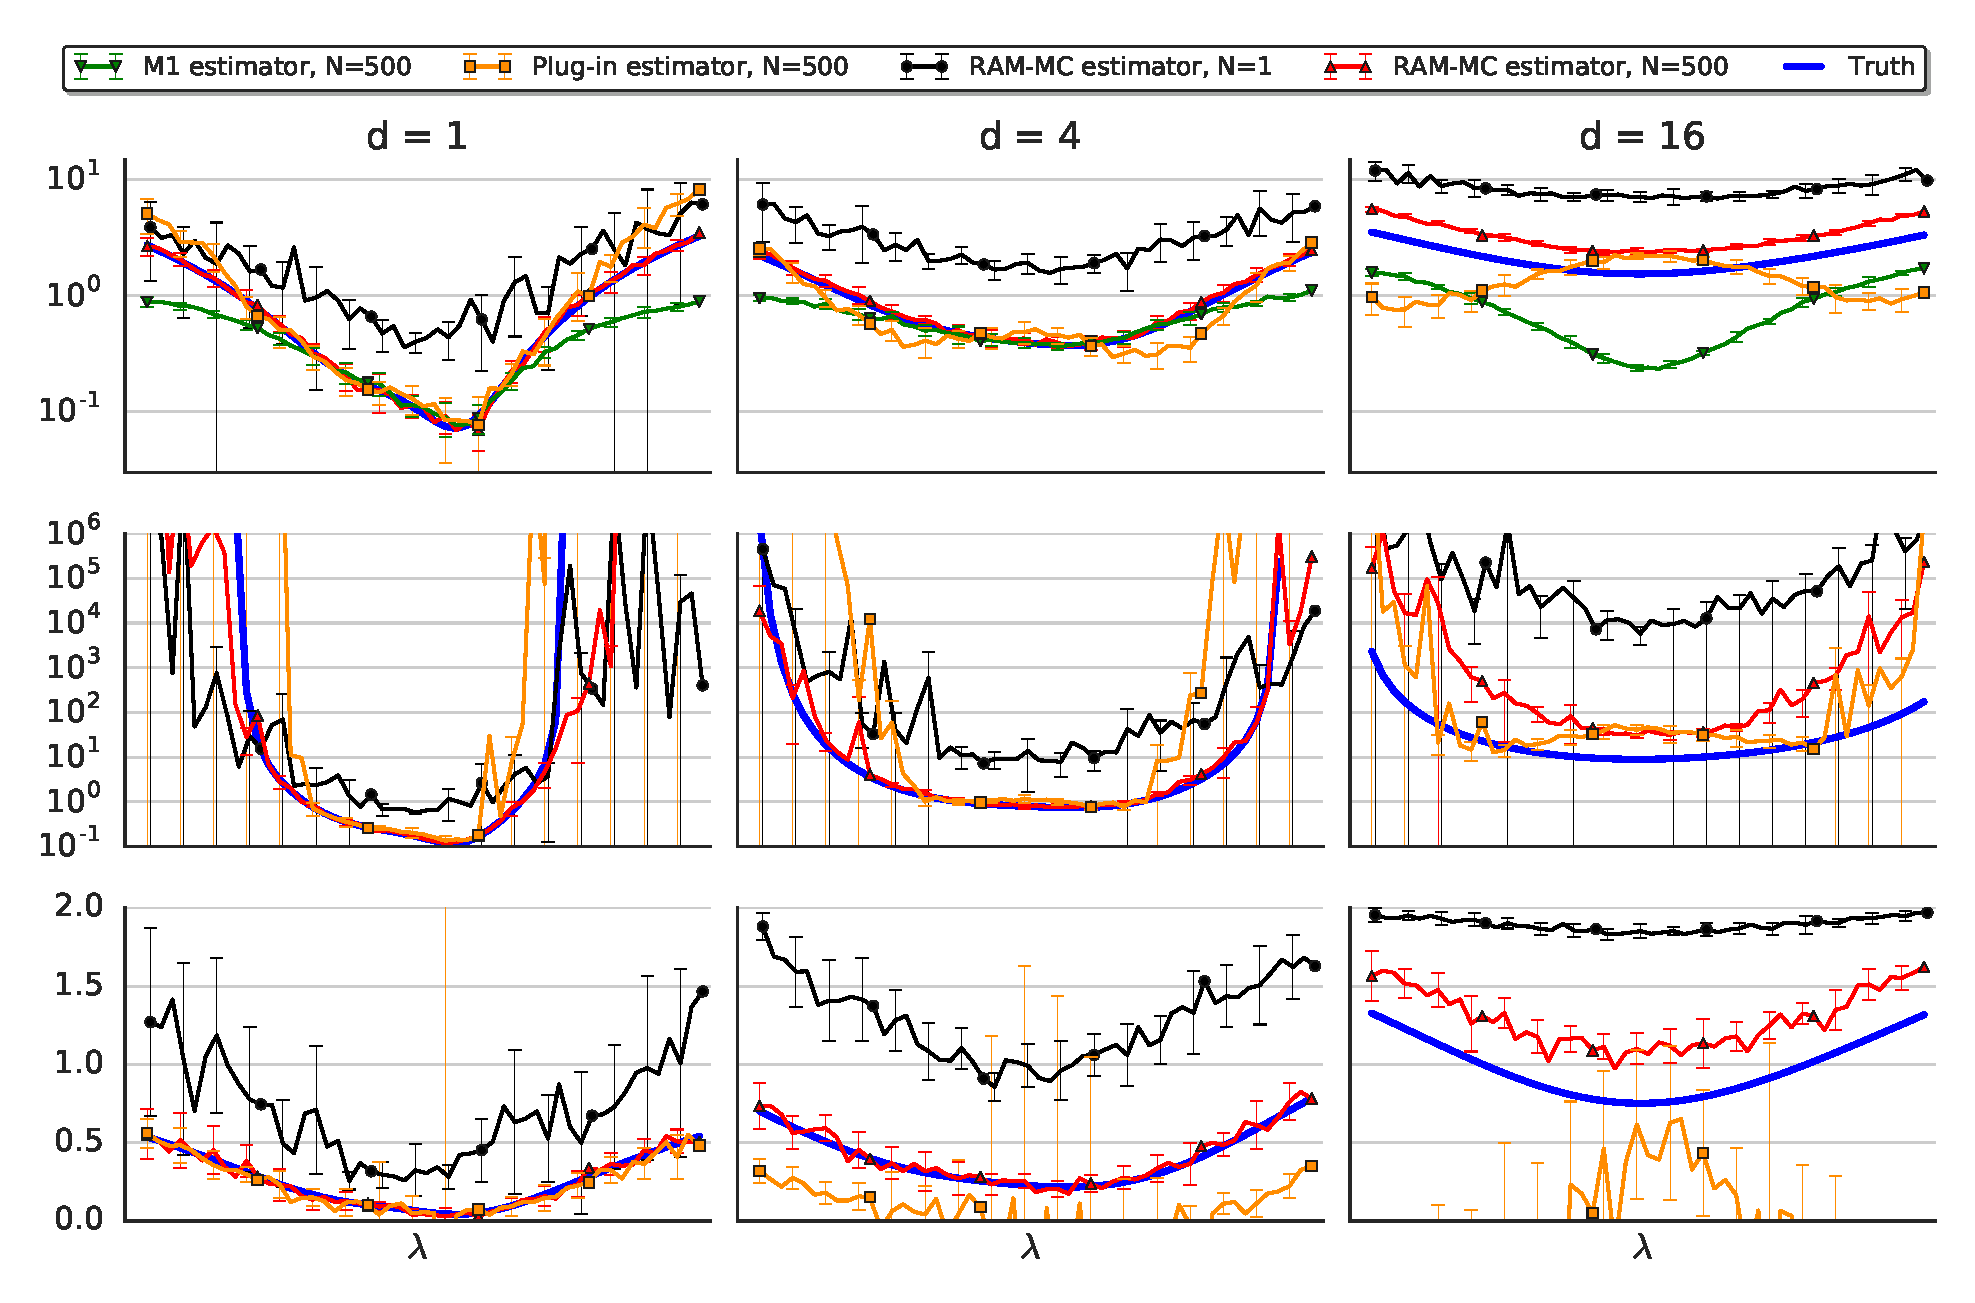
\includegraphics[width=0.97\textwidth, height=0.615\textwidth]{pics/NeurIPS_toy_exps_plot.pdf}};
\node[rotate=0] at (0, 1.7) {$\mathrm{H}^2$};
\node[rotate=0] at (0, 4.2) {$\chi^2$};
\node[rotate=0] at (0, 6.7) {$\mathrm{KL}$};
\end{tikzpicture}
\end{center}
\caption[Evaluation of RAM-MC on synthetic data]{\label{fig:synthetic-exps}
Results of synthetic experiments, Section~\ref{section:synth-exps}.
Estimating $D_f\bigl(\mathcal{N}(\mu_\lambda, \Sigma_\lambda),\, \mathcal{N}(0, I_d)\bigr)$ for various $f$, $d$, and parameters $\mu_\lambda$ and $\Sigma_\lambda$ indexed by $\lambda\in \R$.
Horizontal axis correspond to $\lambda\in[-2, 2]$,
columns to $d\in\{1, 4, 16\}$ and
rows to KL, $\chi^2$, and $\mathrm{H}^2$ divergences respectively.
{\bf \textcolor{blue}{Blue}} are true divergences, 
{\bf black} and {\bf \textcolor{red}{red}} are RAM-MC estimators (Equation \ref{eq:our-mc-estimate}) for $N\in\{1, 500\}$ respectively,
{\bf \textcolor{darkgreen}{green}} are M1 estimator of~\citep{nguyen10ratio} and {\bf \textcolor{orange}{orange}} are plug-in estimates based on Gaussian kernel density estimation \citep{moon14ensemble}.
$N=500$ and $M=128$ in all the plots if not specified otherwise.
Error bars depict one standard deviation over 10 experiments.
}
\end{figure}
\clearpage
}


% and used $\lambda \in [-2,2]$.

%
%Specifically, take ${P_Z} = $ and ${Q_X}$ to be standard normal distributions over $\Z=\R^d$ and $\X=\R^{20}$ respectively,
%and $\smash{Z\sim Q^\lambda_{Z|X}}$ to be a linear transform of $X$ plus a fixed isotropic Gaussian noise, with the linear function parameterised by $\lambda$.
%
%By varying $\lambda$ we can interpolate between different values for $D_f(Q_Z^\lambda , P_Z)$.

%\textbf{The estimators.}
Figure \ref{fig:synthetic-exps} shows the behaviour of RAM-MC with $N\,{\in}\,\{1, 500\}$ and $M{=}128$ compared to the ground truth as $\lambda \in [-2, 2]$ is varied. 
The columns of Figure~\ref{fig:synthetic-exps} correspond to different dimensions $d\,{\in}\,\{1, 4, 16\}$, and rows to the $\KL$, $\chi^2$ and $\mathrm{H}^2$ divergences, respectively. 
For each column, the values of $A_0$ and $v$ were randomly sampled so that the distributions being compared are the same within columns and different between columns.
Two other baseline methods are included for comparison.
First, a plug-in method based on kernel density estimation \citep{moon14ensemble}.
Second, and only for the KL case, the M1 method of \cite{nguyen10ratio} based on density ratio estimation (see Section \ref{sec:literature-density-ratio-estimation}).

%\textbf{The experiment.}
To produce each plot, the following was performed 10 times, with the mean result giving the bold lines and standard deviation giving the error bars.
First, $N$ points $\XN$ were drawn from $Q_X$. 
Then $M{=}128$ points $\ZM$ were drawn from $\hat{Q}_Z^N$ and RAM-MC (Equation \ref{eq:our-mc-estimate}) was evaluated. 
Using $\hat{Q}_Z^N$ as the proposal distribution resulted in significantly better results compared to using $P_Z$ as the proposal distribution for all divergences.
For the plug-in estimator, the densities $\hat{q}(z)$ and $\hat{p}(z)$ were estimated by kernel density estimation with 500 samples from $Q_Z$ and $P_Z$ respectively using the default settings of the Python library {\texttt{scipy.stats.gaussian\_kde}}.
The divergence was then estimated via MC-sampling using $128$ samples from $Q_Z$ and the surrogate densities.
Note that this density estimation approach ignores all of the structure present, and thus demonstrates the poor performance of an agnostic method. 
It would also be possible to exploit part of the problem structure and use one of the known density $p(z)$ or $\widehat{Q}_Z^N$, rather than estimating both by density estimation; these cases led to performance better than the naive density estimation approach, but still significantly worse than RAM-MC and were omitted from Figure \ref{fig:synthetic-exps} to avoid clutter. 
The M1~estimator involves solving a convex linear program in $N$ variables to maximise a lower bound on the true divergence, see \cite{nguyen10ratio} for more details.
Although the M1~estimator can in principle be used for arbitrary $f$-divergences, its implementation requires hand-crafted derivations that are supplied only for the $\KL$ in \cite{nguyen10ratio}.

%\textbf{Discussion.}
The results of this experiment empirically support Proposition \ref{prop:upper-bound} and Theorems \ref{thm:fast-KL-rate}, \ref{thm:convergence-rate-general}, and~\ref{thm:mc-variance}:
(i) in expectation, RAM-MC upper bounds the true divergence; (ii) increasing $N$ from 1 to 500 clearly decreases both the bias and the variance of RAM-MC.
When the dimension $d$ increases, the bias for fixed $N$ also increases.
This is consistent with the theory in that, although the rates are independent of $d$, the constants are not.
By side-stepping the issue of density estimation---that is, samples are drawn at the level of $\mathcal{X}$ so that $Q_Z$ is approximated as a mixture of known components, rather than performing kernel density estimation based on samples at the level of $\mathcal{Z}$---RAM-MC performs favourably compared to the plug-in and M1 estimators, more so in higher dimensions ($d=16$).
In particular, the shape of the RAM-MC curve follows that of the truth for each divergence, while that of the plug-in estimator does not for larger dimensions.
In some cases the plug-in estimator can even take negative values due to the large variance.




\subsection{Real-data experiments}
\label{sec:exp_wae}
%\textbf{The data model.}
To investigate the behaviour of RAM-MC in a more realistic setting, this experiment considers the estimation of divergences in the context of Variational Autoencoders (VAEs) and Wasserstein Autoencoders (WAEs), introduced in Section \ref{sec:literature-gen-models}.
Similar to the synthetic experiments, we are purely concerned with estimating $D_f(Q_Z,P_Z)$ with pre-trained models here, not actually training models from scratch. 
Recall that both VAEs and WAEs have a prior ${P_Z}$ over the latent space and involve learning an encoder $\smash{Q^\phi_{Z|X}}$ with parameter $\phi$ mapping from the data to latent space.
Although the divergence $D_f(Q_Z,P_Z)$ does not appear in the VAE objective function, pretrained VAEs can nonetheless be used alongside WAEs as more realistic, higher dimensional settings to investigate estimation of this quantity compared to the simple synthetic setting considered in the previous section.

%RAM-MC is used to estimate the divergence $D_f(Q^\phi_Z,P_Z)$ between the aggregate posterior and prior.
%A prior distribution ${P_Z}$ is specified, and the 
%optimization objectives of both models are of the form ``reconstruction + distribution matching penalty''.
%The penalty of the VAE was shown by \cite{hoffman2016elbo} to be equivalent to $\smash{\KL(Q^\theta_Z \| P_Z) + I(X,Z)}$ where $I(X,Z)$ is the mutual information of a sample and its encoding.
%The WAE penalty is ${D(Q^\theta_Z \| P_Z)}$ for any divergence $D$ that can practically be estimated.
%Following \cite{tolstikhin2017wasserstein}, we trained models using the Maximum Mean Discrepency (MMD), a kernel-based distance on distributions, and a divergence estimated using a GAN-style classifier leading to WAE-MMD and WAE-GAN respectively \cite{gretton2012kernel, goodfellow2014generative}.
% Both of them can be estimated from samples.
%For more information about VAE and WAE, see Appendix \ref{appendix:intro-vae-wae}.
%\textbf{The experiment.}

Pretrained models that were trained on the \emph{CelebA} dataset \citep{liu2015faceattributes} were used to evaluate the RAM-MC estimator as follows.
The test dataset is taken as the ground-truth $Q_X$, and this is embedded into the latent space via the trained encoder.
Since all models considered have Gaussian encoders, the resulting \emph{empirical aggregate posterior}
is a ${\sim}{20}\text{k}$-component Gaussian mixture for $Q_Z$, one component for each item in the test dataset. 
Since $Q_Z$ is a finite---not continuous---mixture, the true $D_f(Q_Z,P_Z)$ can be estimated using a large number of MC samples ($10^4$ samples were used).
This is computationally costly as it involves evaluating $2\cdot 10^4$ Gaussian densities for each of the $10^4$ MC points.
This evaluation was repeated 10 times, and the means and standard deviations are reported in Figures \ref{fig:real-exps} and \ref{fig:real-exps-hsq} for the KL and $\mathrm{H}^2$ divergences respectively.
RAM-MC is evaluated using $N \in \{2^0, 2^1,\ldots, 2^{14}\}$ and $M \in \{10, 10^3\}$.
For each combination $(N,M)$, RAM-MC was computed 50 times with the means plotted as bold lines and standard deviations as error bars.
This procedure was performed for the KL and $\Hsq$ divergences on six models that were chosen to have latent dimension $d\in\{32, 64, 128\}$ and were selected from the classes VAE, WAE-MMD and WAE-GAN.

\afterpage{%
\begin{figure}
\begin{center}
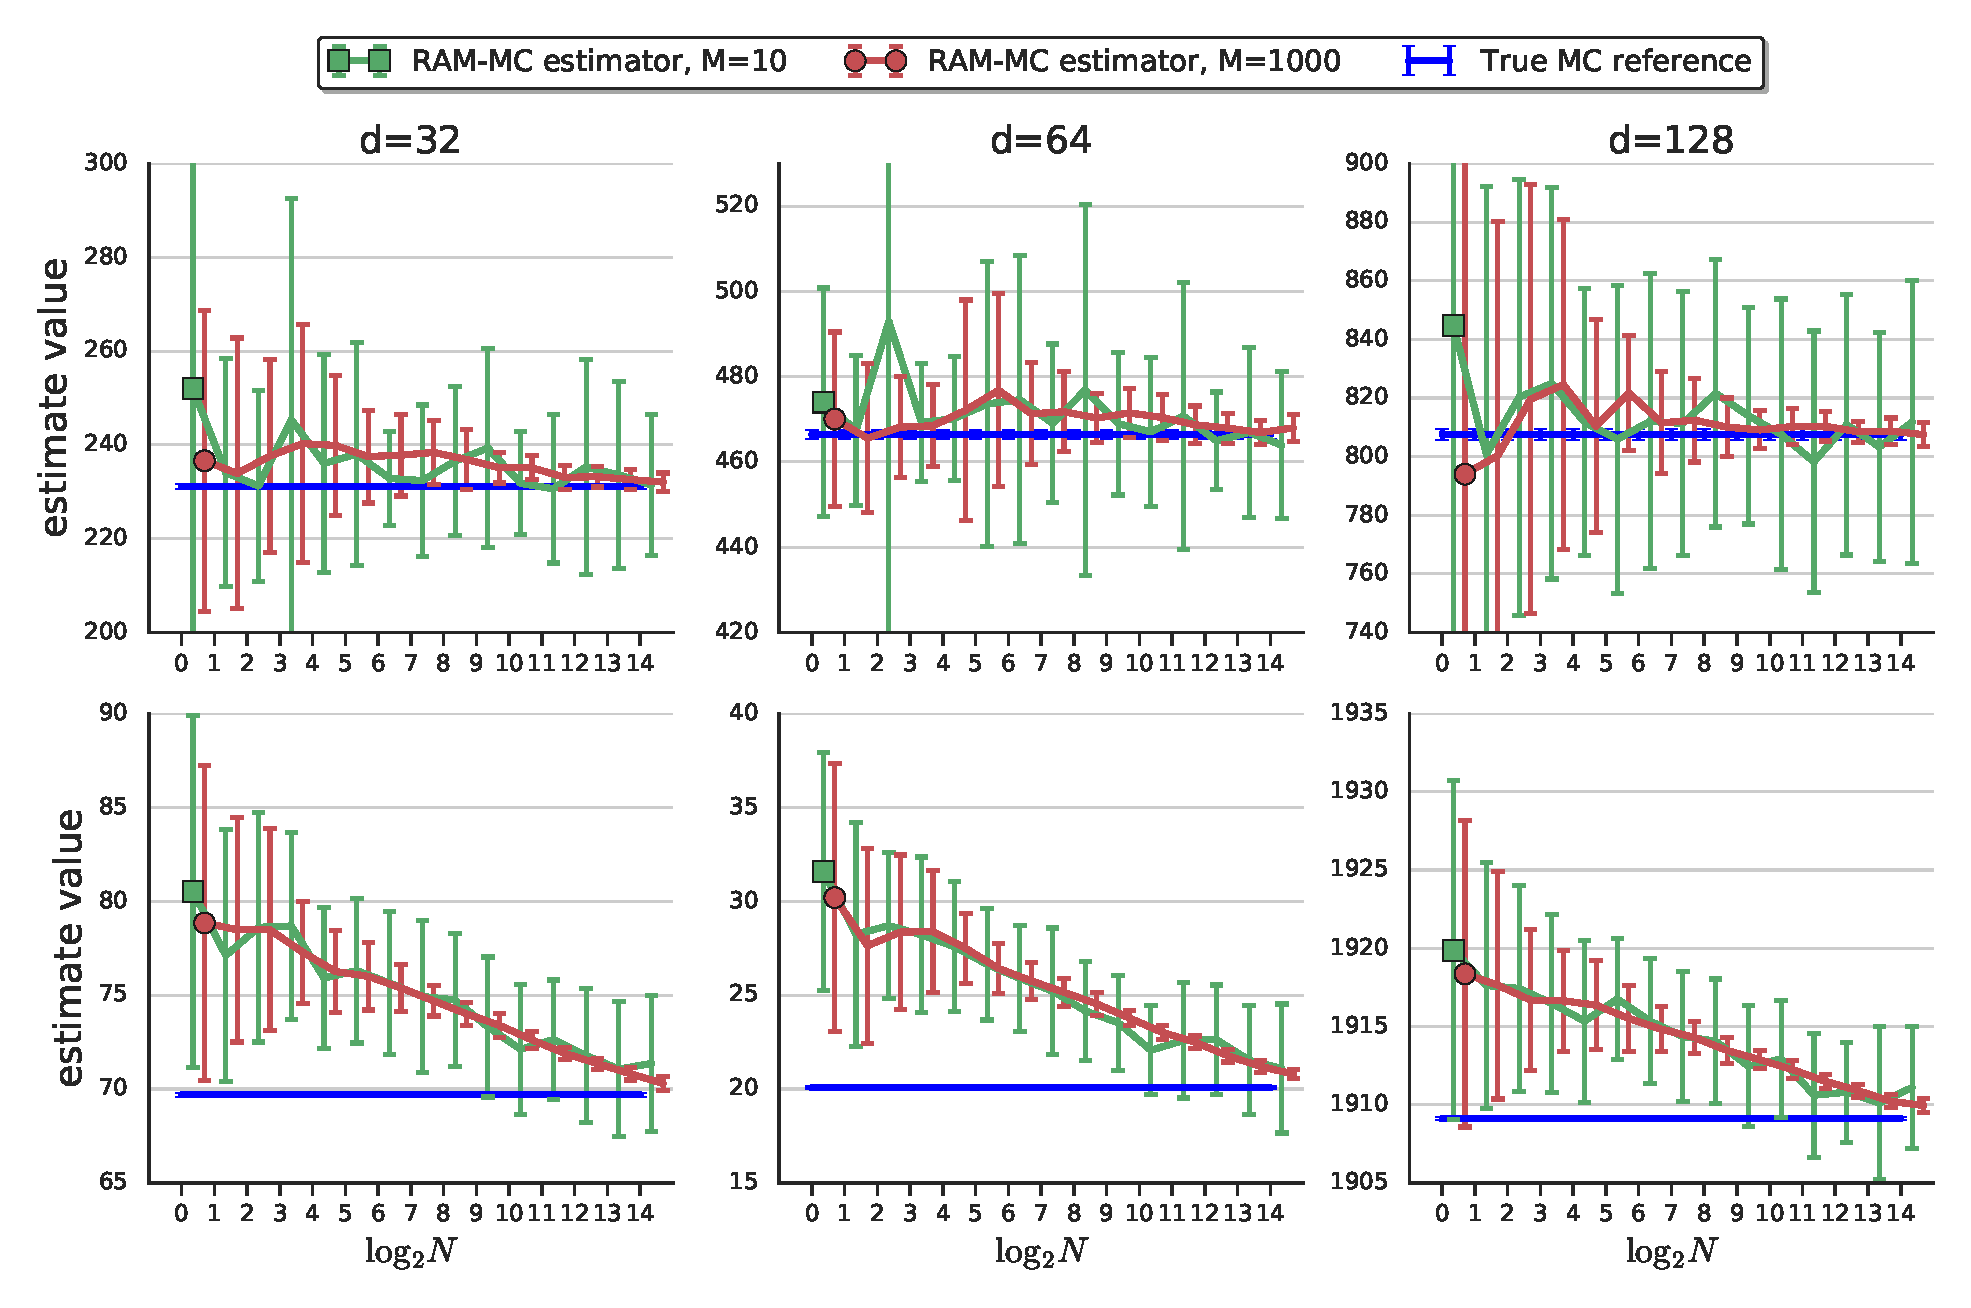
\includegraphics[width=1.\textwidth, height=0.615\textwidth]{pics/NeurIPS_wae_exps_plot.pdf}
\end{center}
\caption[Evaluation of RAM-MC on real data with KL-divergence]{\label{fig:real-exps}
Results of real-data experiments, Section~\ref{sec:exp_wae}. Estimates of $\KL(Q_Z^\theta , P_Z)$ for pretrained autoencoder models with RAM-MC as a function of $N$ for $M{=}10$ ({\bf \textcolor{green!65!blue}{green}}) and $M{=}1000$ ({\bf \textcolor{red}{red}}) compared to an accurate MC estimate of the ground truth ({\bf\textcolor{blue}{blue}}).
Lines and error bars represent means and standard deviations over 50 trials.
}
\end{figure}
\clearpage
}


\afterpage{%
\begin{figure}
\begin{center}
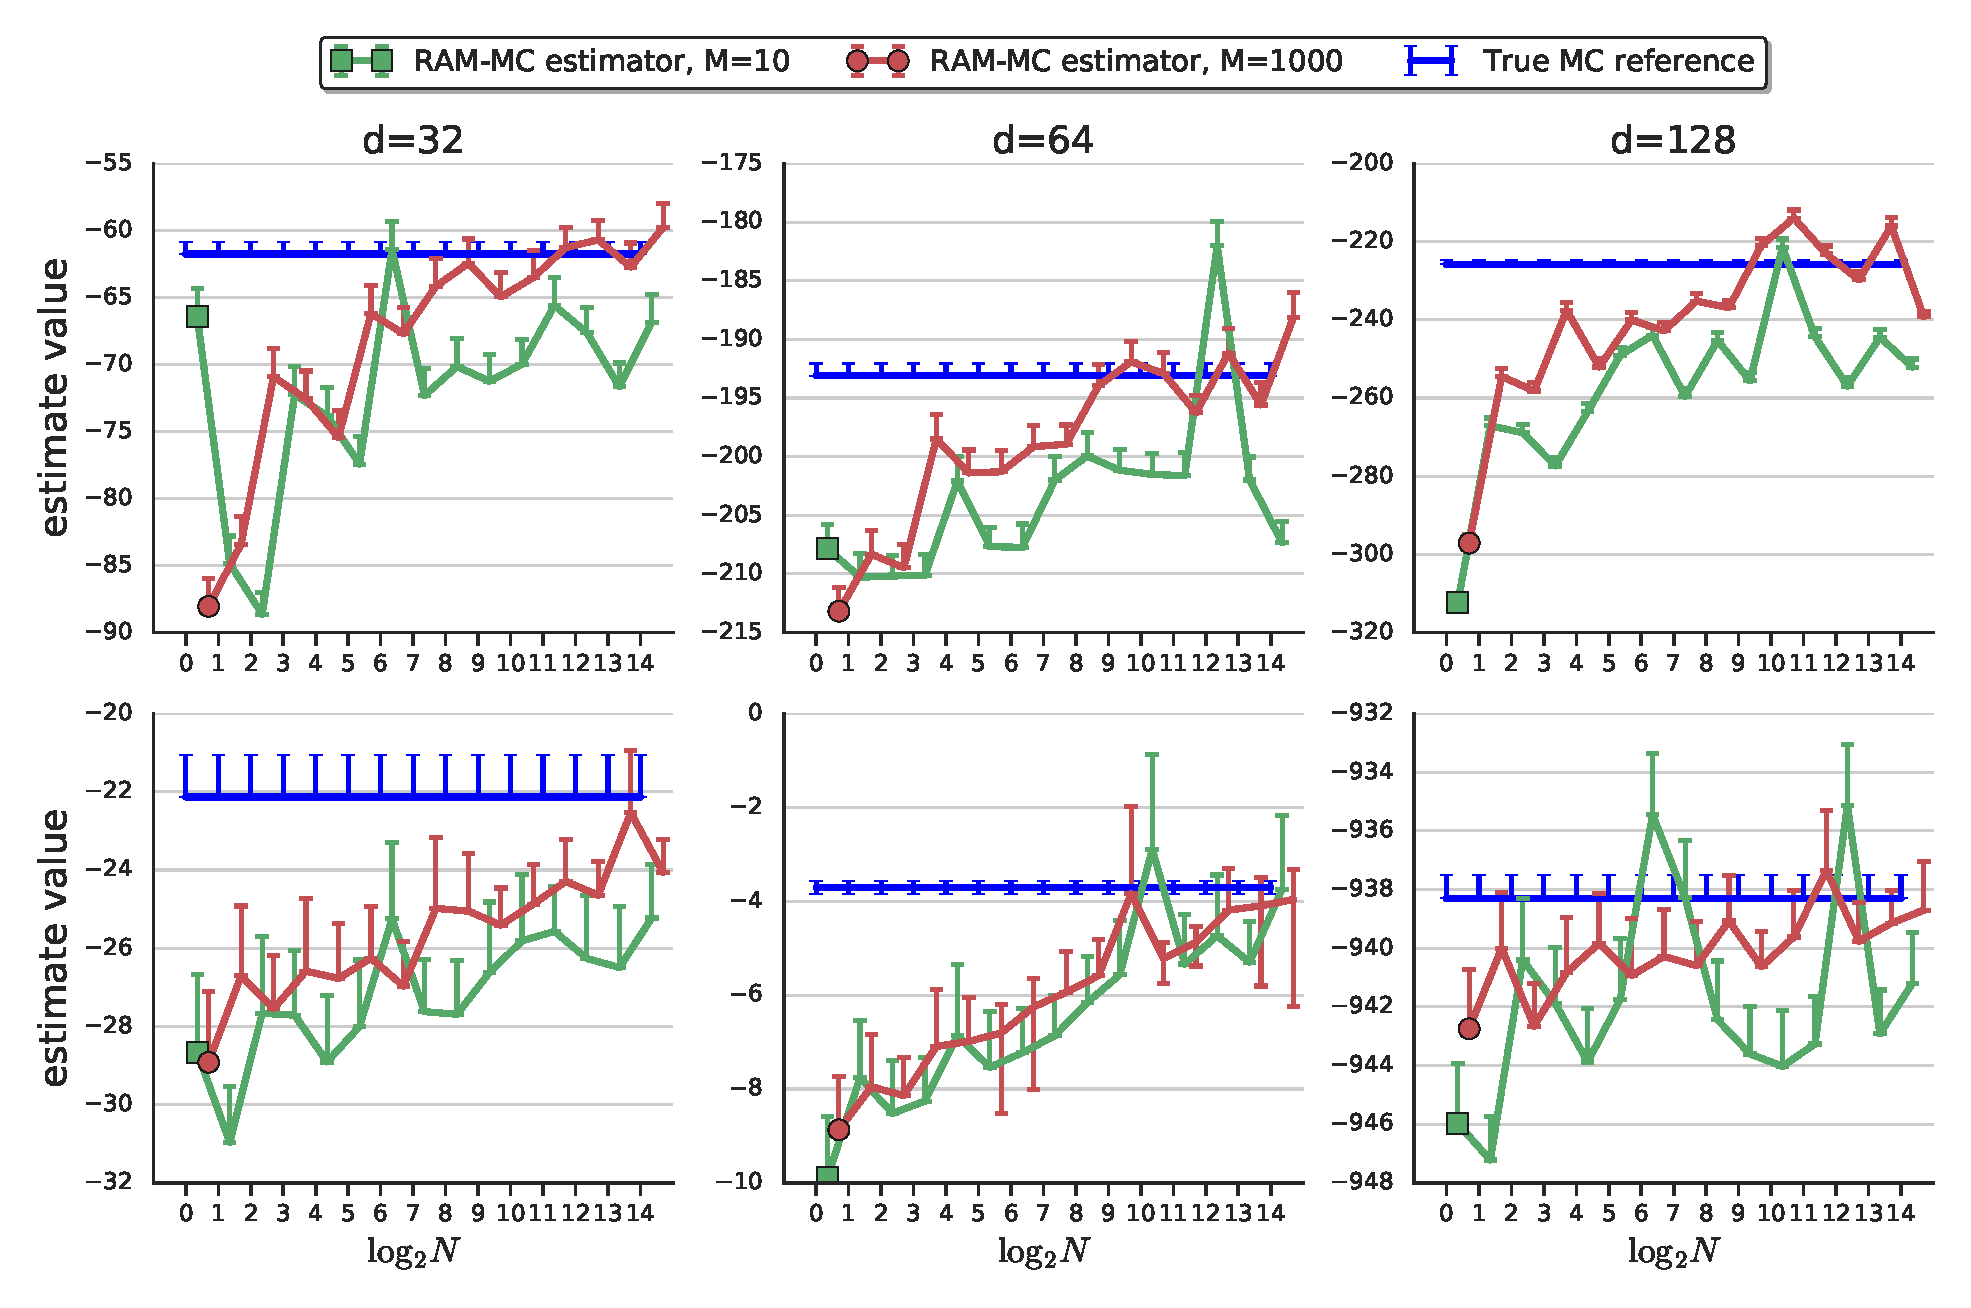
\includegraphics[width=1.\textwidth, height=0.615\textwidth]{pics/NeurIPS_wae_exps_plot_hsq.pdf}
\end{center}
\caption[Evaluation of RAM-MC on real data with $\Hsq$-divergence]{\label{fig:real-exps-hsq}
Results of real-data experiments, Section~\ref{sec:exp_wae}. Estimating $\Hsq(Q_Z^\theta , P_Z)$ in pretrained autoencoder models with RAM-MC as a function of $N$ for $M=10$ ({\bf \textcolor{green!65!blue}{green}}) and $M{=}1000$ ({\bf \textcolor{red}{red}}) compared to ground truth ({\bf\textcolor{blue}{blue}}).
Lines and error bars represent means and standard deviations over 50 trials.
Plots depict $\log\big(2 - \hat{D}^M_{\Hsq}(\hat{Q}^N_Z , P_Z)\big)$ since $\Hsq$ is close to 2 in all models.
Omitted lower error bars correspond to error bars going to $-\infty$ introduced by $\log$.
Note that the approximately \emph{increasing} behaviour evident here corresponds to the expectation of RAM-MC \emph{decreasing} as a function of $N$. 
Due to concavity of $\log$, the decrease in variance when increasing $M$ manifests itself as the {\bf \textcolor{red}{red}} line ($M{=}1000$) being consistently above the {\bf \textcolor{green!65!blue}{green}} line ($M{=}10$).
}
\end{figure}
\clearpage
}

Figure~\ref{fig:real-exps} shows the result of performing this for the KL divergence on six different models.
%For each dimension $d\in\{32, 64, 128\}$, two models were selected from the classes VAE, WAE-MMD and WAE-GAN. 
%See Appendix~\ref{appendix:real-data-experiments-additional} for further details and similar plots for the $H^2$-divergence.
%\textbf{Discussion.}
%The results are encouraging. 
In all cases RAM-MC achieves a reasonable accuracy with $N$ relatively small, even for the bottom right model where the true KL divergence ($\approx 1910$) is large.
There is evidence supporting Theorem~\ref{thm:mc-variance}, which informally states that the variance of RAM-MC is mostly determined by the smaller of $\psi(N)$ and $M$:
when $N$ is small, the variance of RAM-MC does not change significantly with $M$, 
however when $N$ is large, increasing $M$ significantly reduces the variance. 
It was found that there are two general modes of behaviour of RAM-MC across the six trained models considered. 
In the bottom row of Figure~\ref{fig:real-exps}, the decrease in bias with $N$ is very obvious, supporting Proposition~\ref{prop:upper-bound} and Theorems \ref{thm:fast-KL-rate} and \ref{thm:convergence-rate-general}.
In contrast, in the top row it is less obvious, because the comparatively larger variance for $M{=}10$ dominates reductions in the bias.
Even in this case, both the bias and variance of RAM-MC with $M{=}1000$ become negligible for large $N$.
Importantly, the behaviour of RAM-MC does not degrade in higher dimensions.

The baseline estimators (plug-in of \cite{moon14ensemble} and M1 of \cite{nguyen10ratio}) perform so poorly that 
%we decided not to include them in the plots (doing so 
their inclusion would distort the $y$-axis scale.
In contrast, even with a relatively modest $N{=}2^8$ and $M{=}1000$ samples, RAM-MC behaves reasonably well in all cases.

Figure~\ref{fig:real-exps-hsq} displays similar results for the $\Hsq$-divergence.
Since $\Hsq(A,B) \in [0, 2]$ for any probability distributions $A$ and $B$ and all computed estimates were close to $2$,
considerations of scale mean that the estimated values $\log\big(2 - \hat{D}^M_{\Hsq}(\hat{Q}^N_Z , P_Z)\big)$ were plotted instead.
Decreasing bias in $N$ of RAM-MC therefore manifests itself as the lines \emph{increasing} in Figure~\ref{fig:real-exps-hsq}. 
Concavity of $\log$ means that the reduction in variance when increasing $M$ results in RAM-MC with $M{=}1000$ being above RAM-MC with $M{=}10$.
Similar to the results for the KL, these also support the theoretical findings presented in the previous section.

Additionally, the same experiment was attempted using the $\chi^2$-divergence but numerical issues were encountered.
This can be understood as a consequence of the inequality $e^{\KL(A, B)} - 1 \leq \chi^2(A,B)$ for any distributions $A$ and $B$ (Lemma \ref{lemma:f-div-klleqchi}). 
From Figure~\ref{fig:real-exps} it can be seen that the $\KL$-divergence reaches values higher than $1000$, making the corresponding value of the $\chi^2$-divergence larger than can be represented using double-precision floats.






\section{Applications}\label{sec:applications}
This section details some direct consequences of the proposed estimator and its theoretical guarantees to existing literature, illustrating the applicability of this work.
We remind the reader that these results apply specifically to the setting of LVMs with probabilistic encoders.
%In addition, this theory may also apply to a number of machine learning domains where estimating entropy, total correlation or mutual information is either the final goal or part of a broader optimization loop.

\subsection{Entropy estimation}
The differential entropy, defined as $H(Q_Z)= -\int_{\mathcal{Z}} q(z) \log q(z)  dz$, is often a quantity of interest in machine learning.
While it is intractable in general, straightforward computation shows that for \emph{any} $P_Z$
{\addtolength{\abovedisplayskip}{-0.5mm}
\addtolength{\belowdisplayskip}{-0.5mm}
\begin{align*}
    H(&Q_Z) - \mathbb{E}_{\XN} H(\hat{Q}_Z^N) \\
    &= - \int q(z) \log q(z) dz + \mathbb{E}_{\XN} \int \hat{q}_N(z) \log \hat{q}_N(z) dz \\
    &= - \int q(z) \log q(z) dz + \int q(z) \log p(z) dz  \\
    & \qquad - \int \mathbb{E}_{\XN} \hat{q}_N(z) \log p(z) dz  + \mathbb{E}_{\XN} \int \hat{q}_N(z) \log \hat{q}_N(z) dz \\
    &= - \int q(z) \log \frac{q(z)}{p(z)} dz  + \mathbb{E}_{\XN} \int \hat{q}_N(z) \log \frac{\hat{q}_N(z)}{p(z)} dz \\
   	&= \mathbb{E}_{\XN} D_{\text{KL}}\left(\hat{Q}_Z^N , P_Z\right) -  D_{\text{KL}}\left(Q_Z , P_Z\right).
\end{align*}}
Therefore, Theorems \ref{thm:fast-KL-rate} and \ref{thm:convergence-rate-general} provide sufficient conditions under which $\smash{H(\hat{Q}_Z^N)}$ is an asymptotically unbiased estimator of $\smash{H(Q_{Z})}$.
Note that it suffices for the assumptions of these results to hold for \emph{any} choice of $P_Z$, suggesting that a more direct analysis of the behaviour of $\smash{H(\hat{Q}_Z^N)}$ could yield milder sufficient conditions.


\subsection{Total correlation estimation}
The results on entropy estimation have consequences for some existing VAE literature.
The Total Correlation (TC) of a distribution $Q_Z$, defined in terms of the KL-divergence, can be written in terms of differential entropy: 
%
\begin{align*}
TC(Q_Z) &:= D_{\text{KL}}\left(Q_Z, \prod_{i=1}^{d_Z} Q_{Z_i}\right)  \\
&= - \int q(z) \log \left( \frac{q(z)}{\prod_i q(z_i)} \right) dz \\
&= - \int q(z) \log q(z) dz + \int q(z) \sum_i \log q(z_i) dz \\
&= - \int q(z) \log q(z) dz + \sum_i \int q(z_i)  \log q(z_i) dz \\
&= \sum_{i=1}^{d_Z}H(Q_{Z_i}) - H(Q_Z),
\end{align*}
%
where $Q_{Z_i}$ is the $i$th marginal of $Q_Z$.
This is considered by \cite{chen2018isolating}, who subtract it from the VAE loss function (see Section \ref{sec:literature-gen-models}). 
Since a non-negative quantity is subtracted from a lower bound on the evidence, the resulting loss function is still an evidence lower bound, with additional encouragement for $Q_Z$ to be factorised. This is named the $\beta$-TC-VAE algorithm.
By the identities above, estimation of TC can be reduced to estimation of $H(Q_Z)$ with only slight modifications needed to treat $H(Q_{Z_i})$.

Two methods are proposed by \cite{chen2018isolating} for estimating $\smash{H(Q_Z)}$, both of which assume a finite dataset of size $D$.
One of these, named \emph{Minibatch Weighted Sample} (MWS), coincides with $\smash{H(\hat{Q}_Z^N) + \log D}$ estimated with a particular form of MC sampling.
The results presented in this chapter therefore imply \emph{inconsistency} of the MWS method due to the constant $\log D$ offset. 
This inconsistency is fact not problematic in the context of \cite{chen2018isolating} since they are concerned with minimising (not estimating) the TC, and a constant offset does not affect gradient-based optimization techniques.
Interestingly, although their derivations suppose a data distribution of finite support, the results presented here show that minor modifications result in an estimator suitable for both finite and infinite support data distributions.

\subsection{Mutual information estimation}
The mutual information (MI) between variables with joint distribution $\smash{Q_{Z,X}}$ is defined as 
\begin{align*}
\smash{I(Z, X) := D_{\text{KL}}\left(Q_{Z,X}, Q_Z Q_X \right) = \E_{X} D_{\text{KL}}\left(Q_{Z|X}, Q_Z \right)}.
\end{align*}

Several recent papers have estimated or optimised this quantity in the context of autoencoder architectures, coinciding with the setting considered here \citep{hoffman2016elbo, alemi2017fixing, dieng2018avoiding}. 
In particular, \cite{poolevariational} propose the following estimator based on replacing $Q_Z$ with $\smash{\hat{Q}_{Z}^N}$, proving it to be a lower bound on the true MI:
%
\begin{align*}\textstyle
    I_{TCPC}^N(Z,X) = \mathbb{E}_{\XN}\Big[\frac{1}{N} \sum_{i=1}^N D_{\text{KL}}\left( Q_{Z|X_i}, \hat{Q}_{Z}^N \right)\Big] \leq I(Z,X).
\end{align*}
%
The gap in this inequality can be written as
%
\begin{align*}
I(Z,X) - I_{TCPC}^N(Z,X) = \E_{\XN} D_{\text{KL}}\left( \hat{Q}_{Z}^N, P_{Z} \right) - D_{\text{KL}}\left( Q_{Z}, P_Z \right)
\end{align*}
%
where $P_Z$ is \emph{any} distribution. 
Therefore, the results in this chapter also provide sufficient conditions under which $\smash{I^N_{TCPC}}$ is an asymptotically unbiased estimator of the true mutual information.


%\todo{Rewrite section heading to make this next bit fit in, moved from the intro}
\subsection{Related, but fundamentally different work}
\cite{burda2015importance} propose to reduce the gap introduced by Jensen's inequality in the derivation of the classical ELBO by using multiple Monte-Carlo samples from the approximate posterior $\smash{Q_{Z|X}}$.
This is similar in flavour to the approach considered in this chapter, but is fundamentally different since the approach taken here uses multiple samples from the \emph{data distribution} to reduce a different Jensen gap.

To avoid confusion, note that replacing the `regulariser' term $\mathbb{E}_X[D_{\text{KL}}(Q_{Z|X}, P_Z)]$ of the classical ELBO with expectation of the proposed estimator $\E_{\XN}[D_{\text{KL}}(\hat{Q}_Z^N, P_Z)]$ results in an upper bound of the classical ELBO (by Proposition~\ref{prop:upper-bound}) but is itself not in general an evidence lower bound:
%
\begin{align*}
    \mathbb{E}_X \Big[ \mathbb{E}_{Q_{Z|X}} \log p(X|Z) - D_{\text{KL}}(Q_{Z|X}, P_Z ) \Big] \leq \mathbb{E}_X \Big[ \mathbb{E}_{Q_{Z|X}} \log p(X|Z) \Big] - \mathbb{E}_{\XN} \Big[ D_{\text{KL}}(\hat{Q}_Z^N, P_Z ) \Big].
\end{align*}


\section{Conclusion}\label{sec:conclusion}
This chapter introduced a practical estimator for the $\smash{f}$-divergence $D_f(Q_Z,P_Z)$ where $Q_Z = \int Q_{Z|X}dQ_X$, samples from $Q_X$ are available, and $P_Z$ and $Q_{Z|X}$ have known density.
The RAM estimator is based on approximating the true $Q_Z$ with data samples as a random mixture via $\smash{\hat{Q}^N_{Z}=\frac{1}{N}\sum_{n} Q_{Z|X_n}}$,
and RAM-MC is the version of this estimator where $\smash{D_f(\hat{Q}^N_Z,P_Z)}$ is estimated with MC sampling.

Rates of convergence and concentration were proved for both RAM and RAM-MC, in terms of sample size $N$ and MC samples $M$ under a variety of choices of $\smash{f}$.
Due to the strong structural assumptions made on the forms of the distributions in question, the fast rates presented here hold under relatively mild and verifiable further assumptions, thus making them applicable to the estimation of divergences in the latent spaces of autoencoders.
In contrast, in the existing literature on $f$-divergence estimation, which generally makes few structural assumptions, fast rates are only obtained under strong assumptions on the smoothness of densities or density ratios of the distributions. 

Synthetic and real-data experiments strongly support the validity of the proposal in practice, and the theoretical results provide guarantees for methods previously proposed heuristically in existing literature for mutual information and total correlation estimation,
thus extending understanding of the conditions under which these quantities can be estimated with practical numbers of samples.


Future work should investigate the use of the proposals for optimization loops, in contrast to pure estimation.
When $\smash{Q^\phi_{Z|X}}$ depends on parameter $\phi$ and the goal is to minimise $\smash{D_f(Q_Z^\phi , P_Z)}$ with respect to $\phi$, RAM-MC provides a practical surrogate loss that can be minimised using stochastic gradient methods.
The obvious setting to apply this is in training WAEs, where the main problem is minimisation of a divergence term $\smash{D(Q_Z^\phi , P_Z)}$, discussed in Section \ref{subsec:chapter2-wae}.
Indeed, the research presented in this chapter was originally motivated by the study of WAEs.
Preliminary experiements not included in this thesis found little improvement when using RAM-MC as the latent-space matching penalty compared to existing methods (WAE-MMD and WAE-GAN). 
It is possible that this lack of improvement is attributable to deficiencies in the proposed method, or to the use of $f$-divergences in this setting more generally.
It may instead be due to the insufficiently thorough nature of those preliminary experiments.

Another more theoretical direction of research relating the proposed RAM-MC estimator to its application in training WAEs would be to investigate how bounds on the divergence $\smash{D_f(Q_Z^\phi , P_Z)}$ in combination with the reconstruction error of a WAE relate to the optimal transport distance $OT(P^\theta_X, Q_X)$ that a WAE is ultimately supposed to minimise.
Work in this direction has been done by \cite{patrini2018sinkhorn}, who relate the reconstruction error and latent-space optimal transport distance $\smash{OT(Q_Z^\phi , P_Z)}$ with the data-space optimal transport distance $OT(P^\theta_X, Q_X)$. 
However, it is not clear whether such a connection must hold for other choices of latent-space divergences, since the `relaxed' WAE objective (Equation \ref{eq:wae-objective-relaxed}) is itself a heuristic approximation to the original `constrained' optimal transport formulation (Equation \ref{eq:ot-objective-constrained}).




